%!TEX encoding=UTF-8 Unicode
%!TEX encoding=UTF-8 Unicode
%tweeks on pdf version so everybody is happy
\directlua{pdf.setminorversion(4)} % for facile.cines.fr
%\pdfcompresslevel=0 % Not needed

\documentclass[xcolor={usenames,dvipsnames},hyperref={pdfusetitle}]{beamer}
\usepackage{lmodern}
\beamertemplatenavigationsymbolsempty

%=========================Language and encoding ==============================

\usepackage[utf8]{inputenc}
\usepackage[english]{babel}
\usepackage[T1]{fontenc}
% Fix size errors due to T1 in bbl file
\usepackage{fix-cm}
\usepackage{siunitx}
%=============================================================================

%========================= Todo notes  =======================================

%!TEX encoding=UTF-8 Unicode

% Todo notes
\newcommand{\DB}[1]{\todo[author=David,inline]{#1}}
\newcommand{\GH}[1]{\todo[author=Guillaume,inline]{#1}}

% Usefull stuff
\newcommand{\Input}[1]{\input{tex/#1}}

% References
\newcommand{\fig}[1]{Figure~\ref{fig:#1}}
\newcommand{\tbl}[1]{Table~\ref{tab:#1}}
\newcommand{\alg}[1]{Algorithm~\ref{alg:#1}}
\newcommand{\sect}[1]{Section~\ref{sec:#1}}
\newcommand{\chap}[1]{Chapter~\ref{chap:#1}}

% Tools names
\newcommand{\Tabarnac}{\emph{Tabarnac}\xspace}
\newcommand{\Moca}{\emph{Moca}\xspace}


\usepackage{todonotes}
\presetkeys{todonotes}{inline}{}

%=============================================================================

%========================= Figures ===========================================

\usepackage[]{caption}
\usepackage[]{subcaption}
\usepackage{graphicx} % support the \includegraphics command and options
\graphicspath{{./img/}{./style/}{./tikz/}}
%!TEX encoding=UTF-8 Unicode

% Libraries
\usetikzlibrary{shapes,arrows,decorations,decorations.pathreplacing,decorations.markings,fit}
\usetikzlibrary{positioning,backgrounds,calc,patterns}



%!TEX encoding=UTF-8 Unicode
\usepackage{algorithm}
\usepackage{algpseudocode}
\usepackage{varwidth} % for algorithm in tikz node

%\algblockdefx[]{Function}{EndFunction}
%[2]{\algorithmicfunction\ \textproc{#1}{(#2)}}%
%{\algorithmicend\ \algorithmicfunction}%
%\algnewcommand\Callp[2]{\textproc{#1}(#2)}%

\algblockdefx[Program]{Program}{EndProgram}%
    [1]{\texttt{#1:}}%
    {}

\usepackage{listings}

%\renewcommand*\thelstnumber{\arabic{lstnumber}}

\DeclareCaptionFormat{mylst}{\hrule\vspace{1pt}#1#2#3}
\captionsetup[lstlisting]{format=mylst,labelfont=bf,singlelinecheck=off,labelsep=space}
%
\lstset{
    language=C,
    basicstyle=\small\ttfamily,
    numbers=left,
    numbersep=10pt,
    xleftmargin=20pt,
    frame=tb,
    framexleftmargin=20pt,
    escapeinside={|}{|},          % if you want to add LaTeX within your code
    keywordstyle=\bf,
}

% \lstset{ %
%   %backgroundcolor=\color{white},   % choose the background color; you must add \usepackage{color} or \usepackage{xcolor}
%   %basicstyle=\footnotesize,        % the size of the fonts that are used for the code
%   breakatwhitespace=false,         % sets if automatic breaks should only happen at whitespace
%   breaklines=true,                 % sets automatic line breaking
%   captionpos=t,                    % sets the caption-position to bottom
%   %commentstyle=\color{mygreen},    % comment style
%   %deletekeywords={...},            % if you want to delete keywords from the given language
%   escapeinside={|}{|},          % if you want to add LaTeX within your code
%   extendedchars=true,              % lets you use non-ASCII characters; for 8-bits encodings only, does not work with UTF-8
%   frame=tb,	                   % adds a frame around the code
%   keepspaces=true,                 % keeps spaces in text, useful for keeping indentation of code (possibly needs columns=flexible)
%   %keywordstyle=\color{blue},       % keyword style
%   language=C,                 % the language of the code
%   %otherkeywords={*,...},           % if you want to add more keywords to the set
%   numbers=left,                    % where to put the line-numbers; possible values are (none, left, right)
%   numbersep=5pt,                   % how far the line-numbers are from the code
%   numberstyle=\tiny, % the style that is used for the line-numbers
%   rulecolor=\color{black},         % if not set, the frame-color may be changed on line-breaks within not-black text (e.g. comments (green here))
%   showspaces=false,                % show spaces everywhere adding particular underscores; it overrides 'showstringspaces'
%   showstringspaces=false,          % underline spaces within strings only
%   showtabs=false,                  % show tabs within strings adding particular underscores
%   stepnumber=2,                    % the step between two line-numbers. If it's 1, each line will be numbered
%   stringstyle=\color{mymauve},     % string literal style
%   tabsize=2,	                   % sets default tabsize to 2 spaces
%   title=\lstname                   % show the filename of files included with \lstinputlisting; also try caption instead of title
% }

\usepackage{epstopdf}
\usepackage{booktabs}
\usepackage{multirow}
%\usepackage{subcaption}

%=============================================================================

%=============================================================================

%========================= Hyperref ==========================================


%\hypersetup{
%    colorlinks=false, %colore les liens
%    breaklinks=true, %permet le retour à la ligne dans les liens trop longs
%    urlcolor= blue, %couleur des hyperliens
%    %linkcolor= black, %couleur des liens internes
%    bookmarksopen=true,
%    citecolor=black,
%}
%=============================================================================

%========================= Other useful includes =============================

\usepackage{ifthen}
\usepackage[absolute,overlay]{textpos} %to set some blocks position
%=============================================================================

%========================= Beamer theme =====================================

%Stuff for printable version
\mode<handout>{
    \usetheme{default}
    \setbeamercolor{background canvas}{bg=black!5}
    \pgfpagesuselayout{4 on 1}[a4paper,landscape,border shrink=2.5mm]
}

\usetheme{AntibesCompact}

\definecolor{INstruct}{HTML}{82A382}
\setbeamercolor{structure}{fg=INstruct}


%=============================================================================

%========================= Title frame  ======================================
\title[]{Analyzing the memory behavior of parallel scientific applications}
\author[David Beniamine]{\textbf{David Beniamine}}
\institute[Polaris / Datamove]{
    
\includegraphics[height=.10\textheight]{img/logoUGA.jpg}
    \quad
    
\includegraphics[width=.10\textwidth]{img/LIG_coul.jpg}
    \quad
    
\includegraphics[width=.15\textwidth]{img/inria.jpg}
    \quad
    
\includegraphics[width=.18\textwidth]{img/polaris.png}
    \quad
    
\includegraphics[width=.18\textwidth]{img/datamove.png}
}

\newcommand{\enableTocAtSection}{
    \AtBeginSection[]
    {
        \ifthenelse{\boolean{sectiontoc}}{
            \begin{frame}<beamer>
                \frametitle{Outline}
                \tableofcontents[currentsection,currentsubsection]
            \end{frame}
        }
    }
    \AtBeginSubsection[]
    {
        \ifthenelse{\boolean{sectiontoc}}{
            \ifthenelse{\thesubsection>1}{
                \begin{frame}<beamer>
                    \frametitle{Outline}
                    \tableofcontents[currentsection,currentsubsection]
                \end{frame}
            }
        }
    }
}

%=============================================================================

\begin{document}
%========================= Title and outlines ================================
\begin{frame}{}
    \titlepage
\small
{\centering\itshape Jury members\par}
\begin{tabular}[t]{@{}l@{\hspace{3pt}}p{.45\textwidth}@{}}
President: & Pr, Martin Quinson\\
Reviewers: & Pr, Jes\'us Labarta Mancho \\
& Pr,  Raymond Namyst \\
Examiners: & Dr, Lucas M. Schnorr \\
\end{tabular}%
\begin{tabular}[t]{@{}l@{\hspace{3pt}}p{.45\textwidth}@{}}
Supervisors: & Pr, Bruno Raffin \\
 & Dr, Guillaume Huard
\end{tabular}%
\end{frame}

\newboolean{sectiontoc}
\setboolean{sectiontoc}{true} % default to true

%=============================================================================

%========================= Real presentation =================================

\begin{section}{Context}

\begin{frame}{Science and computers}
    %!TEX encoding=UTF-8 Unicode

% Layers

\definecolor{Computer}{HTML}{D95F02}
\definecolor{Science}{HTML}{1B9E77}
\definecolor{Theory}{HTML}{7570B3}

\tikzstyle{arr}  = [-latex,very thick]
\tikzset{
  filled box/.style = {
    shape = rectangle,
    draw  = #1,
    fill  = #1,
    text width=6em,
    rounded corners},
}

%\newlength{\cornerlength}
%\setlength{\cornerlength}{.1}

\begin{tikzpicture}[font=\small,scale=1]
    \node[text=white,filled box=Computer] (computers)   at (0,3) {\only<5->{\textbf{More\newline performant\newline}} Computers};
    \uncover<2->{
        \node[text=white,filled box=Science] (simu)        at (5,5) {\only<4->{\textbf{More complex\newline}} Simulations \newline and large scale \newline experiments};
        \path[arr,Computer] (computers.north) edge[out=90,in=180] (simu.west);
}
    \uncover<3->{
        \node[text=white, filled box=Theory] (th)          at (8,0)  {New theories\newline and hypothesis};
        \path[arr,Science] (simu.east) edge[out=0,in=90] (th.north);
    }

    \uncover<4->{
        \path[arr,Theory] (th.west) edge[out=180,in=-75] (simu.south);
    }
 
    \uncover<5->{
        \path[arr,Science] (simu.south) edge[out=-105,in=0] (computers.east);
    }


\end{tikzpicture}
% vim: et si sta lbr  sw=4 ts=4 spelllang=en_us

\end{frame}

\begin{frame}{Improving sequential computers performances}
    \begin{columns}
        \begin{column}{.45\textwidth}
            \centering
            %!TEX encoding=UTF-8 Unicode
%Palette GnBu 5 col + white
\definecolor{ColPU}{HTML}{FFFFFF}
\definecolor{ColCore}{HTML}{F0F9E8}
\definecolor{ColL1}{HTML}{BAE4BC}
\definecolor{ColL2}{HTML}{7BCCC4}
\definecolor{ColL3}{HTML}{43A2CA}
\definecolor{ColM}{HTML}{0868AC}
\definecolor{ColS}{HTML}{FFFFFF}

\pgfdeclarelayer{bg}
\pgfdeclarelayer{bbg}
\pgfdeclarelayer{bbbg}
\pgfsetlayers{bbbg,bbg,bg,main}


\tikzset{
    box/.style={
        shape=rectangle,
        text centered,
        draw,
    },
}

\begin{tikzpicture}[font=\small, every pic/.style={scale=.9}]
    \node[box,fill=ColPU] (PU-0) at (0,0) {Thread};
    \node[minimum width=3.3em] (name) at ($(PU-0)+(0,1)$) {Core};

    \begin{pgfonlayer}{bg}
        \node[box,fill=ColCore, fit=(name) (PU-0) ] (core-0) {};
    \end{pgfonlayer}

    \node (cache) at ($(core-0.north)+(0,1)$) {};

    \uncover<4->{
        \draw (core-0.north) -- (cache);

        \draw[fill=ColL3] ($(core-0.north west)+(0,.5)$) rectangle
            ($(core-0.north east)+(0,1)$) node[pos=.5] {Cache};
    }

    \node (cpu-name) at ($(cache)+(0,.5)$) {CPU};

    \begin{pgfonlayer}{bbg}
        \node[box,fill=ColS,fit=(core-0) (cpu-name)] (cpu) {};
    \end{pgfonlayer}

    \draw[line width=.5em] (cpu.north) -- ($(cpu.north)+(0,1)$);

    \draw[fill=ColM, text=white] ($(cpu.north west)+(-.5,1)$) rectangle
        ($(cpu.north east)+(.5,2)$) node[pos=.5]{Memory};


\end{tikzpicture}
% vim: et si sta lbr  sw=4 ts=4 spelllang=en_us

            \begin{block}{}
                \only<1-2>{
                    Before 1990
                }
                \uncover<3->{
                    Early 90's
                }
            \end{block}
        \end{column}
        \begin{column}{.45\textwidth}
            \pause
            \begin{block}{Increase CPU frequency}
                \begin{itemize}
                    \item Gap CPU / Memory
                    \item Energy consumption
                \end{itemize}
            \end{block}
            \pause
            \begin{alertblock}{Memory}
                \begin{itemize}
                    \item Spatial locality
                    \item Temporal locality
                    \item Caches
                \end{itemize}
            \end{alertblock}
            \pause
            \begin{alertblock}{Energy}
                Build parallel machines
            \end{alertblock}
        \end{column}
    \end{columns}
\end{frame}

\begin{frame}{Parallel and NUMA machines}
    \begin{columns}
        \begin{column}{.2\linewidth}
            \begin{block}{}
                \alt<1>{
                    Early 2000's
                }{
                    2007 - Now
                }
            \end{block}
        \end{column}
        \begin{column}{.8\linewidth}
            \centering
            \scalebox{.6}{
                %!TEX encoding=UTF-8 Unicode
%Palette GnBu 5 col + white
\definecolor{ColPU}{HTML}{FFFFFF}
\definecolor{ColCore}{HTML}{F0F9E8}
\definecolor{ColL1}{HTML}{BAE4BC}
\definecolor{ColL2}{HTML}{7BCCC4}
\definecolor{ColL3}{HTML}{43A2CA}
\definecolor{ColM}{HTML}{0868AC}
\definecolor{ColS}{HTML}{FFFFFF}

\pgfdeclarelayer{bg}
\pgfdeclarelayer{bbg}
\pgfdeclarelayer{bbbg}
\pgfsetlayers{bbbg,bbg,bg,main}


\tikzset{
    box/.style={
        shape=rectangle,
        text centered,
        draw,
    },
    pics/core/.style args={#1#2#3#4}{
        % Args: #1: nb PU, #2 core id, #3 direction: + or -
        code={
            \pgfmathtruncatemacro{\pmin}{#1*#2}
            \pgfmathtruncatemacro{\pmax}{\pmin+#1-1}
            %PUs
            \foreach \pu in {\pmin,...,\pmax}{
                \pgfmathtruncatemacro{\pstep}{\pu-\pmin}
                \node[box,fill=ColPU] (PU-\pu)at (0,#3.7*\pstep) {PU\#\pu};
            }
            %Core ID
            \node (inv) at ($(PU-\pmin)#3(0,-.3)$) {};
            \node[minimum width=3.3em] (name) at ($(PU-\pmin)!0.5!(PU-\pmax)#3(0,1)$) {Core\##2};
            % L1
            \begin{pgfonlayer}{bg}
                \node[box,fill=ColCore,inner sep=.1pt, fit=(name) (PU-\pmin)
                (PU-\pmax) (inv)] (core-#2) {};
            \end{pgfonlayer}
            \draw[fill=ColL1] ($(core-#2.#4 west)#3(0,.1)$) rectangle ($(core-#2.#4 east)#3(0,.5)$)%
            node[pos=.5] (l1) {L1};
            % links
            \draw (core-#2.#4) -- ($(core-#2.#4)#3(0,.1)$);
            \coordinate (l1-#2-n) at ($(core-#2.#4)#3(0,.5)$);
        }
    },
    pics/l2group/.style args={#1#2#3#4}{
        % Args: #1: nb Cores, #2 group id, #3 direction: + or -
        code={
            \pgfmathtruncatemacro{\cmin}{#1*#2}
            \pgfmathtruncatemacro{\cmax}{\cmin+#1-1}
            % Cores
            \foreach \core in {\cmin,...,\cmax}{
                \pgfmathtruncatemacro{\cstep}{\core-\cmin}
                \draw (1.4*\cstep,0) pic[font=\tiny] {core={2}{\core}{#3}{#4}};
            }
            % L2
            \draw[fill=ColL2] ($(core-\cmin.#4 west)#3(0,.6)$) rectangle
            ($(core-\cmax.#4 east)#3(0,1.1)$) node[pos=.5]{L2};
            % Coordinates for L3
            \coordinate (l2g-#2-w) at ($(core-\cmin.#4 west)#3(0,1.1)$);
            \coordinate (l2g-#2-e) at ($(core-\cmax.#4 east)#3(0,1.1)$);
            %links
            \foreach \core in {\cmin,...,\cmax}{
                \draw (l1-\core-n) -- ($(core-\core.#4)#3(0,.6)$);
            }
        }
    },
    pics/socket/.style args={#1#2#3#4}{
        % Args: #1: nb l2 groups, #2 socket id, #3 arguments for underlying pics
        code={
            \pgfmathtruncatemacro{\lmin}{#1*#2}
            \pgfmathtruncatemacro{\lmax}{\lmin+#1-1}
            % Cores
            \foreach \lg in {\lmin,...,\lmax}{
                \pgfmathtruncatemacro{\lgstep}{\lg-\lmin}
                \draw (2.8*\lgstep,0) pic[font=\small] {l2group={2}{\lg}{#3}{#4}};
            }
           % L3
            \draw[fill=ColL3] ($(l2g-\lmin-w)#3(0,.1)$) rectangle ($(l2g-\lmax-e)#3(0,.5)$)%
            node[pos=.5]{L3};
           % Coordinates for Mem
            \coordinate (s-#2-w) at ($(l2g-\lmin-w)#3(0,.5)$);
            \coordinate (s-#2-e) at ($(l2g-\lmax-e)#3(0,.5)$);
           % links
           %\foreach \lg in {\lmin,...,\lmax}{
           %    \draw ($(l2g-\lg-w)!.5!(l2g-\lg-e)$) --
           %        ($(l2g-\lg-w)!.5!(l2g-\lg-e)#3(0,.1)$);
           %}
           % CPU
            \ifthenelse{\equal{#3}{+}}{
                \node (minnode) at (-.6,-.3) {};
            }{
                \node (minnode) at (-.6,.3) {};
            }
            \node (maxnode) at ($(l2g-\lmax-e)#3(0,1)$) {};
            \node (sockname) at ($(l2g-\lmin-e)#3(0,.8)$) {Socket \##2};

            \begin{pgfonlayer}{bbg}
                \node[box,fill=ColS,fit=(minnode) (maxnode)] (cpu-#2) {};
            \end{pgfonlayer}
           % Memory
            \draw[fill=ColM,text=white] ($(cpu-#2.#4 west)#3(0,.5)$) rectangle ($(cpu-#2.#4 east)#3(0,1.5)$)%
            node[pos=.5]{Memory bank \##2};

            \draw[very thick] (cpu-#2.#4) -- ($(cpu-#2.#4)#3(0,.5)$);

        }
    },
}

\begin{tikzpicture}[font=\small, every pic/.style={scale=.9}]
    \pic at (0,0)  {socket={2}{0}{+}{north}};
    \pic at (6.5,0)  {socket={2}{1}{+}{north}};
    \pic at (0,-2) {socket={2}{2}{-}{south}};
    \pic at (6.5,-2) {socket={2}{3}{-}{south}};

    \begin{pgfonlayer}{bbbg}
        \draw[line width=1em] (cpu-0) -- (cpu-2);
        \draw[line width=1em] (cpu-0) -- (cpu-1);
        \draw[line width=.3em]  (cpu-0) -- (cpu-3);
        \draw[line width=1em] (cpu-1) -- (cpu-3);
        \draw[line width=1em] (cpu-2) -- (cpu-3);
        \draw[line width=.3em]  (cpu-1) -- (cpu-2);
    \end{pgfonlayer}

\end{tikzpicture}
% vim: et si sta lbr  sw=4 ts=4 spelllang=en_us

            }
        \end{column}
    \end{columns}
\end{frame}

\begin{frame}{Sequential matrix multiplication}
    \centering
    \scalebox{.6}{
        %!TEX encoding=UTF-8 Unicode
%Palette PuOr 4 cols
\definecolor{ColI}{HTML}{1B9E77}
\definecolor{ColJ}{HTML}{D95F02}
\definecolor{ColK}{HTML}{7570B3}

\pgfdeclarelayer{background}
\pgfdeclarelayer{foreground}
\pgfsetlayers{background,foreground}


\tikzstyle{PrimaryA}   = [-latex,very thick]
\tikzstyle{SecondaryA} = [-latex,very thick,dashed]
\tikzstyle{SwapA} = [latex-latex, thick,dotted]

\newcommand{\coli}[1]{\textcolor{ColI}{#1}}
\newcommand{\colj}[1]{\textcolor{ColJ}{#1}}
\newcommand{\colk}[1]{\textcolor{ColK}{#1}}

\tikzset{
    algorithm/.style={
        shape=rectangle,
        alias=this,
        append after command = {
            \pgfextra{
              % Top and bottom lines
                \draw [] ($(this.north west)+(0,.5)$) -- ($(this.north east)+(0,.5)$);
                \node [anchor=west] at ($(this.north west)+(0,0.25)$) {\textbf{Algorithm} #1};
                \draw [] (this.north west) -- (this.north east);
                \draw [] (this.south west) -- (this.south east);
            }
        }
    },
    matgrid/.style args={#1#2}{
        %#1: name #2: size
        alias=this,
        append after command ={
            \pgfextra{
                \draw (this) grid ($(this)+(#2,#2)$);
                % Four corners
                \coordinate (m#1-00) at ($(this)+(0.5,0.5)$);
                \coordinate (m#1-0N) at ($(this)+(0.5,#2-0.5)$);
                \coordinate (m#1-N0) at ($(this)+(#2-0.5,0.5)$);
                \coordinate (m#1-NN) at ($(this)+(#2-0.5,#2-0.5)$);

                \node (#1) at ($(m#1-00)+(-1,0)$){\textbf{#1}};

                \node at ($(m#1-0N)+(-.2,.2)$)  {0};
                \node at ($(m#1-00)+(0,-.2)$) {N-1};
                \node at ($(m#1-NN)+(0,0)$)  {N-1};

            }
        }
    }
}



\begin{tikzpicture}[font=\Large]

    \begin{pgfonlayer}{background}
        \node[algorithm=Matrix multiplication] at (0,8.5){%
            \begin{varwidth}{\linewidth}
                \begin{algorithmic}
                    \For{\coli{i in 0..N-1}}
                    \alt<1-6>{
                        \For{\colj{j in 0..N-1}}
                        \For{\colk{k in 0..N-1}}
                    }{
                        \For{\colk{k in 0..N-1}}
                        \For{\colj{j in 0..N-1}}
                    }
                    \State C[\coli{i},\colj{j}] += A[\coli{i},\colk{k}] * B[\colk{k},\colj{j}]
                            \EndFor
                        \EndFor
                    \EndFor
                \end{algorithmic}%
            \end{varwidth}%
        };

        \coordinate (cj) at (-2.7,9.7);
        \coordinate (cjint) at (-3.8,9.7);
        \coordinate (ckint) at (-3.8,9.1);
        \coordinate (ck) at (-2,9.1);
        \uncover<7->{
            \path[draw,SwapA] (cj) .. controls (cjint) and (ckint) ..(ck);
        }

        \uncover<2->{
            \node[matgrid={A}{5}] at (0,0){};
        }
        \uncover<5->{
            \node[matgrid={B}{5}] at (7,6){};
        }
        \uncover<4->{
            \node[matgrid={C}{5}] at (7,0){};
        }

    \end{pgfonlayer}

    % Indexes

    \begin{pgfonlayer}{foreground}
        %% A
        \uncover<2->{
            \draw[PrimaryA,ColK]   (mA-0N) -- node [above] {\textbf{k}} (mA-NN);
        }
        \uncover<3->{
            \draw[SecondaryA,ColI] (mA-0N) -- node [left]  {\textbf{i}} (mA-00);
            \foreach \i in {1,...,4}{
                \draw[PrimaryA,ColK]   ($(mA-0N)+(0,-\i)$) -- ($(mA-NN)+(0,-\i)$);
            }
        }

        %% B
        \uncover<5-6>{
            \draw[PrimaryA,ColK]   (mB-0N) -- node(bk) [left]  {\textbf{k}} (mB-00);
        }
        \uncover<6>{
            \draw[SecondaryA,ColJ] (mB-0N) -- node(bj) [above] {\textbf{j}} (mB-NN);
            \foreach \i in {1,...,4}{
                \draw[PrimaryA,ColK]   ($(mB-0N)+(\i,0)$) -- ($(mB-00)+(\i,0)$);
            }
        }

        \uncover<7->{
            \draw[PrimaryA,ColJ] (mB-0N) -- node(bj) [above] {\textbf{j}} (mB-NN);
            \draw[SecondaryA,ColK]   (mB-0N) -- node(bk) [left]  {\textbf{k}} (mB-00);
            \foreach \i in {1,...,4}{
                \draw[PrimaryA,ColJ]   ($(mB-0N)-(0,\i)$) -- ($(mB-NN)-(0,\i)$);
            }
        }

        %% C
        \uncover<4->{
            \draw[PrimaryA,ColJ]   (mC-0N) -- node [above] {\textbf{j}} (mC-NN);
            \draw[SecondaryA,ColI] (mC-0N) -- node [left]  {\textbf{i}} (mC-00);
            \foreach \i in {1,...,4}{
                \draw[PrimaryA,ColJ]   ($(mC-0N)+(0,-\i)$) -- ($(mC-NN)+(0,-\i)$);
            }
        }
    \end{pgfonlayer}

\end{tikzpicture}
% vim: et si sta lbr  sw=4 ts=4 spelllang=en_us

    }
\end{frame}

\begin{frame}{Alignment}
    \hspace{-40pt}
    \scalebox{.8}{
        %!TEX encoding=UTF-8 Unicode
%Palette PurOr 4 Col
\definecolor{ColG}{HTML}{5E3C99}
\definecolor{ColB}{HTML}{FDB863}

\newcommand{\colg}[1]{\textcolor{ColG}{#1}}
\newcommand{\colb}[1]{\textcolor{ColB}{#1}}

\pgfdeclarelayer{bg}
\pgfsetlayers{bg,main}


\tikzstyle{arr}   = [-latex,thick]
\tikzstyle{txtnode} = [anchor=west]
\tikzstyle{mybrace} = [decorate,decoration={brace, mirror,amplitude=1em},thick]
\tikzstyle{mydash} = [dashed, dash pattern=on 1pt off 2pt]

\def\eltsz{3}
\def\vshift{-1.5}
\def\balign{.6}
\pgfmathparse{\balign*\eltsz}
\edef\balignsz{\pgfmathresult}
\def\nlines{1}
\pgfmathparse{\nlines-\balign}
\edef\resid{\pgfmathresult}

\tikzset{
    myarray/.style args={#1#2#3#4}{
        % args: size-1, fill, show number ?
        alias=this,
        append after command = {
            \pgfextra{
                \coordinate (#4-base) at ($(this.west)+(0,\vshift)$);
                \pgfmathparse{#1-1}
                \foreach \i in {0,...,\pgfmathresult}{
                    \draw[fill=#2] ($(#4-base)+(\eltsz*\i,0)$) rectangle ($(#4-base)+(\eltsz*\i+\eltsz,1)$);
                    \ifthenelse{#3=0}{}{
                        \node[anchor=south] at ($(#4-base)+(\eltsz*\i,1)$) {\i};
                    }
                }
                \ifthenelse{#3=0}{}{
                    \node[anchor=south] at ($(#4-base)+(\eltsz*#1,1)$){#1};
                }
            }
        }
    },
}



\begin{tikzpicture}[font=\small]
    \node[myarray={4}{none}{1}{bad},txtnode] (bad) at (0,0) {\colb{\textbf{Bad alignment:}}};

    \begin{pgfonlayer}{bg}
        \node[myarray={2}{ColG,mydash}{0}{invb},txtnode] (d0) at (\balignsz,0) {};
        \path[pattern=north east lines, pattern color=ColB] (0,\vshift) rectangle ($(0,\vshift)+(\balignsz,1)$);
        \path[pattern=north east lines, pattern color=ColB] (\balignsz+\eltsz*2,\vshift) rectangle (3*\eltsz,1+\vshift);
    \end{pgfonlayer}

    \draw[mybrace] (0,\vshift) -- (1*\eltsz,\vshift) node [midway,below=1em]
        {Fetch 0};
    \draw[mybrace] (\eltsz,\vshift) -- (2*\eltsz,\vshift) node [midway,below=1em]
        {Fetch 1};

    \draw[mybrace] (2*\eltsz,\vshift) -- (3*\eltsz,\vshift) node [midway,below=1em]
        {Fetch 2};

    \node[anchor=west] at (0,2*\vshift)
    {\textbf{Total:} \colb{3 fetches}, \colg{2~useful lines} / \colb{1~useless line}};

    %% Good alignment
    \node[myarray={4}{none}{1}{good},txtnode] (good) at (0,3*\vshift) {\colg{\textbf{Good alignment:}}};

    \begin{pgfonlayer}{bg}
        \node[myarray={2}{ColG,mydash}{0}{invg},txtnode] (d1) at (0,3*\vshift) {};
    \end{pgfonlayer}

    \draw[mybrace] (0,\vshift+3*\vshift) -- (\eltsz,\vshift+3*\vshift) node
        [midway,below=1em] {Fetch 0};
    \draw[mybrace] (\eltsz,\vshift+3*\vshift) -- (2*\eltsz,\vshift+3*\vshift) node
        [midway,below=1em] {Fetch 1};
    \node[anchor=west] at (0,5*\vshift)
    {\textbf{Total:} \colg{2 fetches}, \colg{2~useful lines} / \colb{0~useless lines}};

\end{tikzpicture}
% vim: et si sta lbr  sw=4 ts=4 spelllang=en_us

    }
    \begin{block}{Cache lines}
        \begin{itemize}
            \item Memory split into cache lines (64 bytes)
            \item One access retrieves a whole line
        \end{itemize}
    \end{block}
\end{frame}

\begin{frame}{False sharing}
    \hspace{-35pt}
    \scalebox{.8}{
        %!TEX encoding=UTF-8 Unicode

\definecolor{Col0}{HTML}{1B9E77}
\definecolor{Col1}{HTML}{D95F02}

%\newcommand{\col0}[1]{\textcolor{Col0}{#1}}
%\newcommand{\col1}[1]{\textcolor{Col1}{#1}}

\pgfdeclarelayer{bg}
\pgfsetlayers{bg,main}


\tikzstyle{arr}   = [-latex,very thick]
\tikzstyle{txtnode} = [anchor=west]

\def\eltsz{1.5}
%\def\balign{.4}
%\def\nlines{2}
%\pgfmathparse{\nlines-\balign}
%\edef\resid{\pgfmathresult}

\tikzset{
    myarray/.style args={#1#2}{
        % args: size-1
        alias=this,
        append after command = {
            \pgfextra{
                \coordinate (base) at (this.west);
                \foreach \i in {0,...,#1}{
                    \draw[fill=#2] ($(base)+(\eltsz*\i,0)$) rectangle ($(base)+(\eltsz*\i+\eltsz,1)$);
                }
            }
        }
    },
}



\begin{tikzpicture}[font=\small]
    \node[myarray={7}{none}] (cache) at (0,0) {};
    \draw[arr,Col0] (.5,.5) -- node[above,pos=.5] {Thread 0} (4*\eltsz-.5,.5);
    \draw[arr,Col1] (4*\eltsz+.5,.5) -- node[above,pos=.5] {Thread 1} (8*\eltsz-.5,.5);
\end{tikzpicture}
% vim: et si sta lbr  sw=4 ts=4 spelllang=en_us

    }
    \begin{block}{Cache line (64 bytes)}
        \begin{itemize}
            \item Consistency handled at cache line level
            \item<alert@1-> Conflict on parallel write
            \item Conflict freeze cache hierarchy
        \end{itemize}
    \end{block}
\end{frame}

\begin{frame}{Summary}
    \begin{block}{Issues}
        \begin{itemize}
            \item Order of accesses
            \item Alignment
            \item False sharing
            \item Thread and data placement
            \item Remote NUMA accesses
        \end{itemize}
    \end{block}
    \pause
    \begin{alertblock}{Real applications}
        \begin{itemize}
            \item Complex data structures
            \item Memory accesses patterns hard to identify from code
            \item Thread handled by high level libraries
        \end{itemize}
    \end{alertblock}
\end{frame}

\begin{frame}{Research statement}
    \begin{alertblock}{}
        How can we analyze the memory behavior of an application to optimize its performances ?
    \end{alertblock}
    \pause
    \begin{block}{Challenges}
        \begin{enumerate}
                \item Collect memory traces
                \begin{itemize}
                    \item \textbf{Complete}: do not miss part of the address space
                    \item \textbf{Precise}:  enough to detect patterns
                    \item \textbf{Detailed}: embed time, space, location, nature
                \end{itemize}
                \item Visualize memory traces
                \item Optimize applications using the obtained knowledge
        \end{enumerate}
    \end{block}
\end{frame}

\end{section}

\begin{frame}{Outline}
    \tableofcontents
\end{frame}

\section{Related work}
\enableTocAtSection

\begin{frame}{Trace collection mechanisms}
    \begin{block}{Performance counters}
        \begin{itemize}
            \item Hardware based / lightweight
            \item CPU point of view
        \end{itemize}
    \end{block}
    \pause
    \begin{block}{Instrumentation}
        \begin{itemize}
            \item Flexible
            \item Usually slow
            \item Vendor specific libraries: Intel Pin~\cite{Luk05Pin}
        \end{itemize}
    \end{block}
    \pause
    \begin{alertblock}{Instruction sampling~\cite{Drongowski07Instructionbased,Levinthal09Performance}}
        \begin{itemize}
            \item Lightweight
            \item Detailed information on memory
            \item Coarse grain sampling
        \end{itemize}
    \end{alertblock}
\end{frame}

\begin{frame}{Existing memory profiling tools}
    \begin{block}{}
        \begin{itemize}
            \item  MemPhis~\cite{McCurdy10Memphis}
            \item<alert@1->  MemProf~\cite{Lachaize12MemProf}
            \item  HPCToolkit extension~\cite{Liu14Tool}
            \item <alert@1-> MemAxes / Mitos~\cite{Gimenez14Dissecting}
        \end{itemize}
    \end{block}
    \pause
    \begin{alertblock}{Limitations}
        \begin{itemize}
            \item Not complete: miss significant part of memory
            \item Not precise enough to detect patterns
        \end{itemize}
    \end{alertblock}
\end{frame}

\section{Tabarnac: Analyzing the global memory behavior}

\subsection{Design}

\begin{frame}{Main principles}
    \begin{block}{Goals}
        \begin{itemize}
            \item Global understanding of memory behavior
            \item Designed for NUMA machines
            \item Focus on thread sharing and data mapping
            \item Simple to use
        \end{itemize}
    \end{block}
    \pause
    \begin{alertblock}{Mechanism}
        Pin instrumentation
    \end{alertblock}
\end{frame}

\begin{frame}{Background knowledge}
    \begin{block}{Mapping tools}
        \begin{itemize}
            \item Dynamic tools~\cite{Corbet12Toward,Diener14kMAF}
                \begin{itemize}
                    \item Collect informations on memory accesses online
                    \item Move data close to thread using them
                \end{itemize}
            \item  Static policies
                \begin{itemize}
                    \item First touch (default)
                    \item Interleave: reduce memory contention
                \end{itemize}
        \end{itemize}
    \end{block}
    \pause
    \begin{alertblock}{Numalyze~\cite{Diener15Characterizing}}
        \begin{itemize}
            \item Pin~\cite{Luk05Pin} instrumentation, lock free
            \item Intercept every memory accesses
            \item Collects one counter per page and per thread
            \item Designed to compare dynamic mapping tools
        \end{itemize}
    \end{alertblock}
\end{frame}

\begin{frame}{Tabarnac}
    \begin{alertblock}{}
        \begin{itemize}
            \item Build on top of Numalyze
            \item Differentiate access types (reads / writes)
            \item Retrieve data structure information
                \begin{itemize}
                    \item Read binary for static data structures
                    \item Intercepts allocations
                    \item Uses debug flags to decide data structure names
                \end{itemize}
            \item R visualizations
            \item Filter out almost unused data structures
        \end{itemize}
    \end{alertblock}
\end{frame}

\subsection{Optimizing IS, a well known benchmark}

\begin{frame}{IS}
    \begin{block}{}
        \begin{itemize}
            \item NAS Parallel Benchmark~\cite{Jin99NPBOpenMP}
            \item Integer (bucket) Sort
            \item Memory Intensive
            \item<alert@1-> “Random memory access” (according to NPB website)
        \end{itemize}
    \end{block}
\end{frame}

\begin{frame}{Data structures}
    \begin{columns}
        \begin{column}{.45\linewidth}
            \centering
            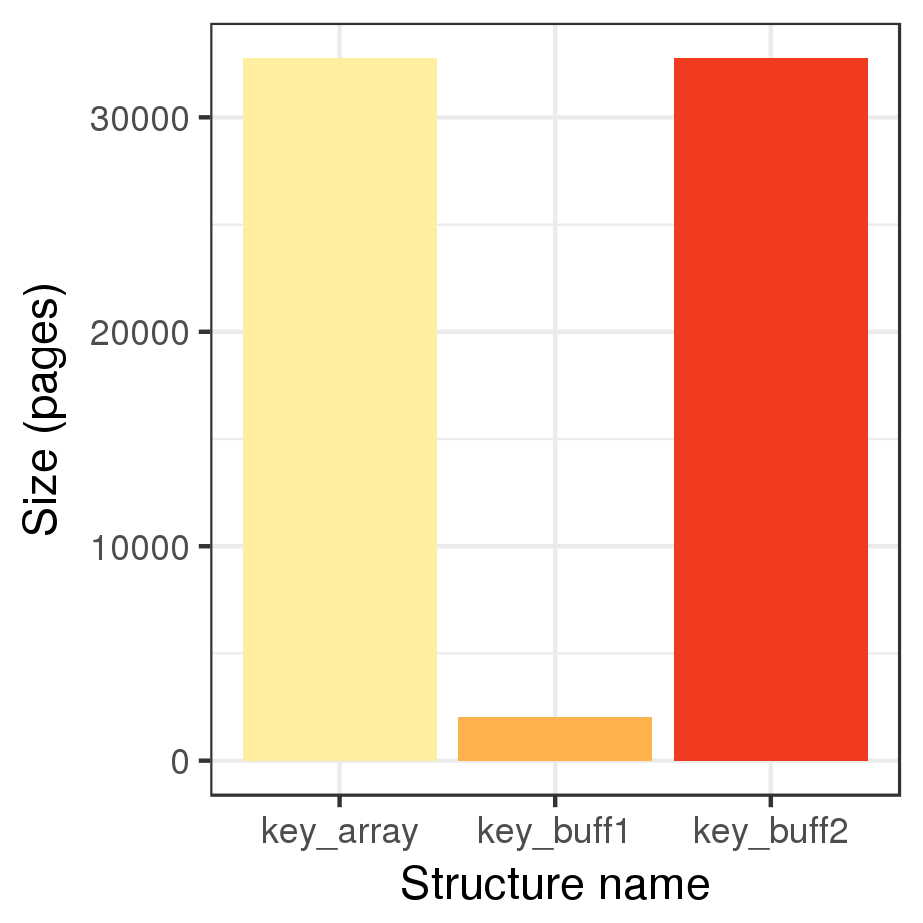
\includegraphics[width=\linewidth]{tabarnac/is_b_structs_sz.png}
        \end{column}
        \begin{column}{.45\linewidth}
            \centering
            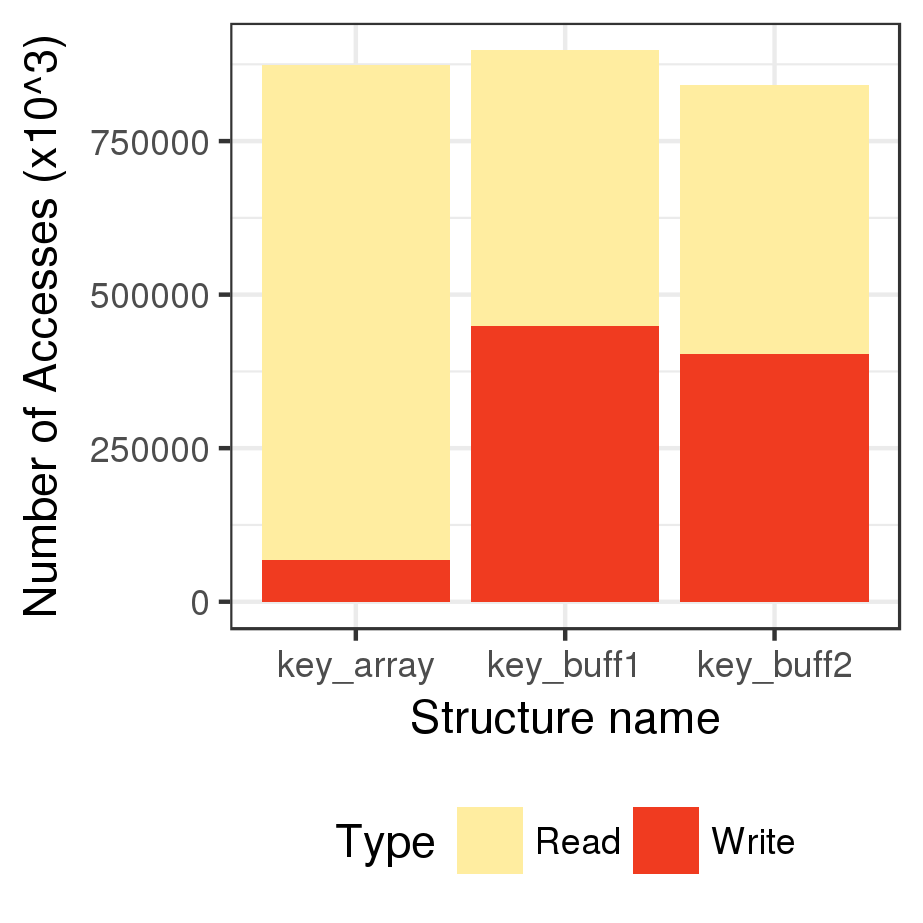
\includegraphics[width=\linewidth]{tabarnac/is_b_structs_rw.png}
        \end{column}
    \end{columns}
\end{frame}

\begin{frame}{First touch}
    \alt<1>{
        \begin{columns}
            \begin{column}{.45\linewidth}
                \centering
                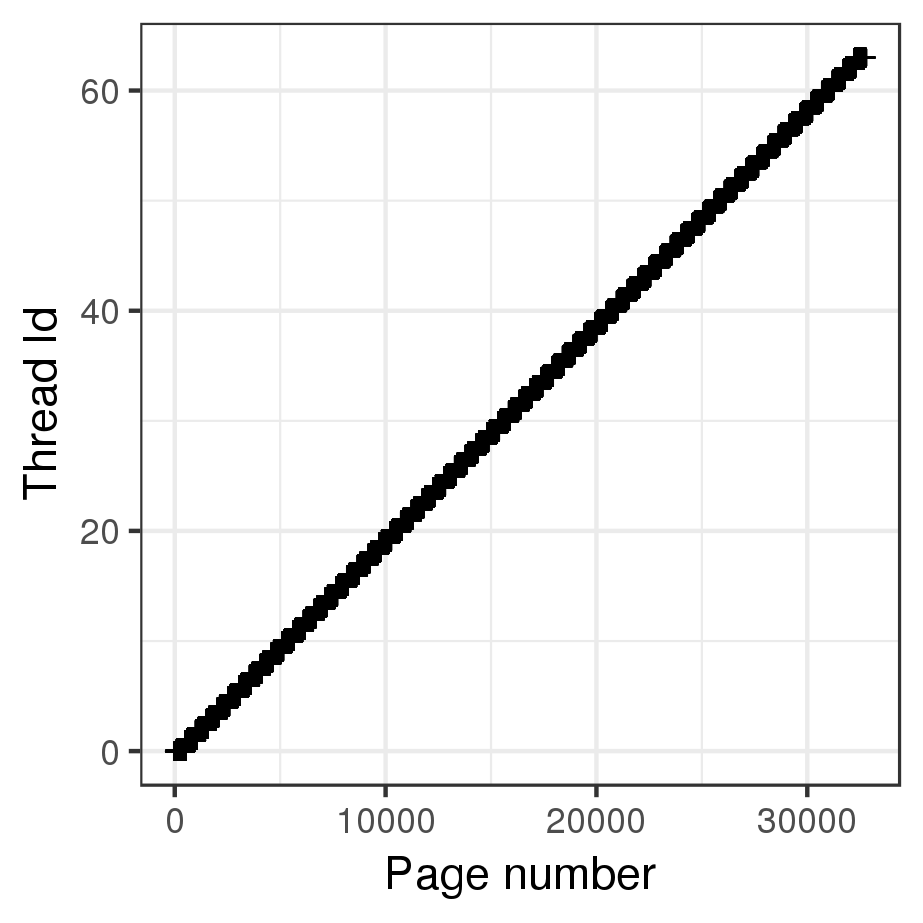
\includegraphics[width=\linewidth]{tabarnac/is_b_ka_ft.png}
            \end{column}
            \begin{column}{.45\linewidth}
                \centering
                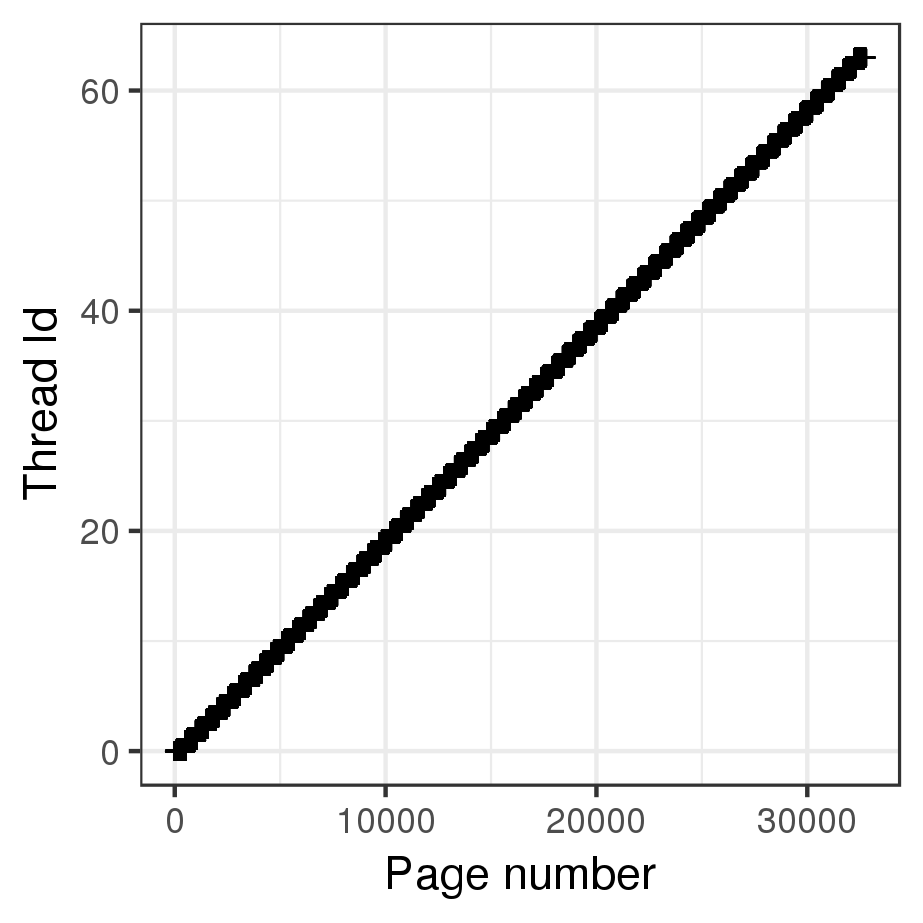
\includegraphics[width=\linewidth]{tabarnac/is_b_kb2_ft.png}
            \end{column}
        \end{columns}
    }{
        \centering
        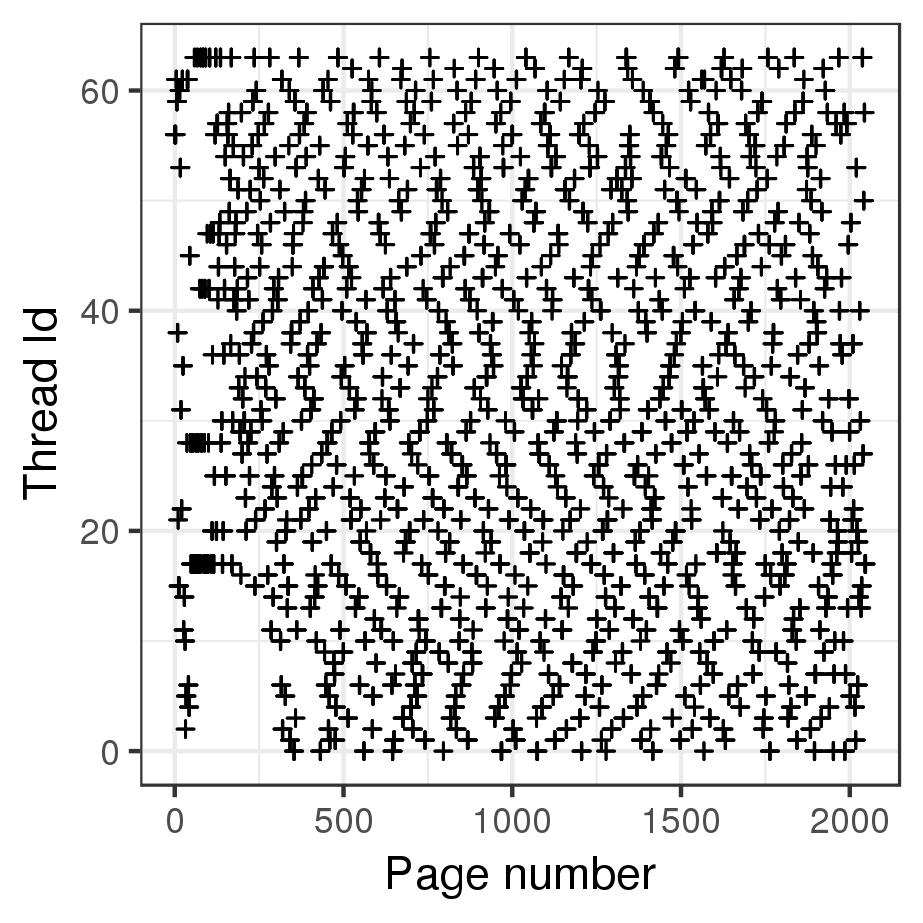
\includegraphics[width=.65\linewidth]{tabarnac/is_b_kb1_ft.png}
    }
    \pause
\end{frame}

\begin{frame}{Accesses distribution}
    \alt<1>{
        \begin{columns}
            \begin{column}{.45\linewidth}
                \centering
                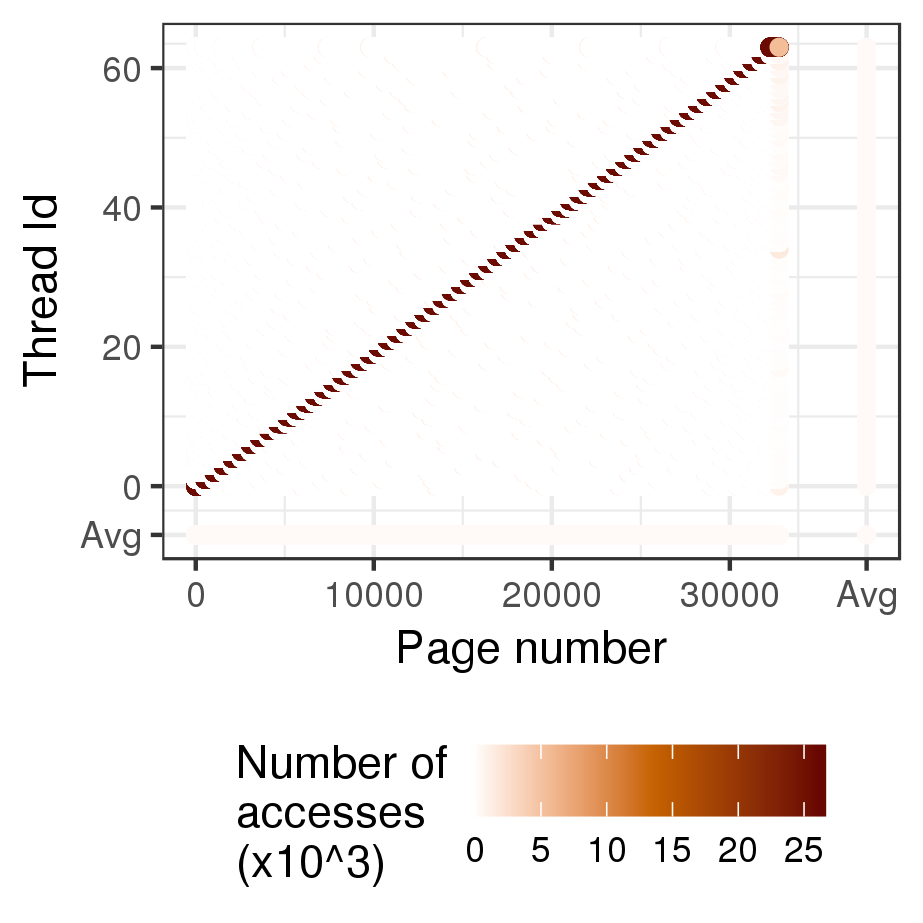
\includegraphics[width=\linewidth]{tabarnac/is_b_ka_dist.png}
            \end{column}
            \begin{column}{.45\linewidth}
                \centering
                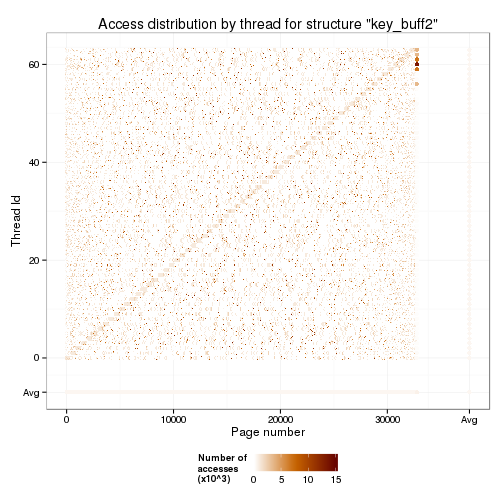
\includegraphics[width=\linewidth]{tabarnac/is_b_kb2_dist.png}
            \end{column}
        \end{columns}
    }{
        \centering
        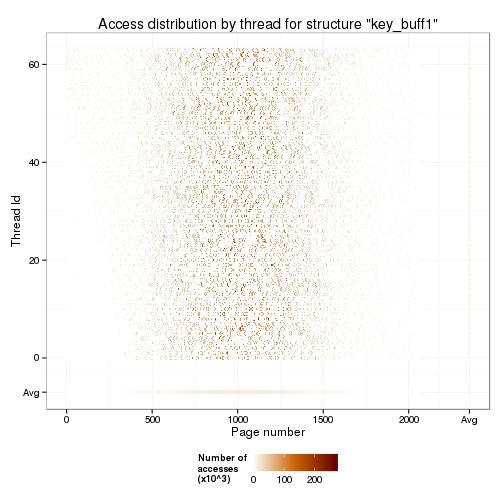
\includegraphics[width=.65\linewidth]{tabarnac/is_b_kb1_dist.png}
    }
    \pause
\end{frame}

\begin{frame}{Understanding and fixing the issue}
    \centering
    \alt<1>{
        \includegraphics[height=.6\textheight]{standalone/is-curve-nocolor}
    }{
        \alt<2>{
            \includegraphics[height=.6\textheight]{standalone/is-curve-random}
        }{
            \alt<3>{
                \includegraphics[height=.6\textheight]{standalone/is-curve-cyclic}
            }{
            \includegraphics[height=.6\textheight]{standalone/is-curve}
            }
        }
    }
    \begin{block}{\uncover<2->{
            \alt<1-2>{
                Dynamic scheduling
            }{
                \alt<3>{
                    Cyclic scheduling
                }{
                    Fair scheduling
                }}}}
        \uncover<2->{\alert{
        \#pragma omp for schedule
            \alt<1-2>{
                (dynamic)\\
            }{
                \alt<3>{
                    (static)\\
                }{
                    (static, size/(2*num\_threads))\\
                }
            }
            }}
        for (k=0;k<N;k++)\\
            \qquad key\_buff1[key\_buff2[k]]++
    \end{block}
    \pause
    \pause
    \pause
\end{frame}

\begin{frame}{Modified accesses distribution}
    \alt<2>{
        \begin{columns}
            \begin{column}{.45\linewidth}
                \centering
                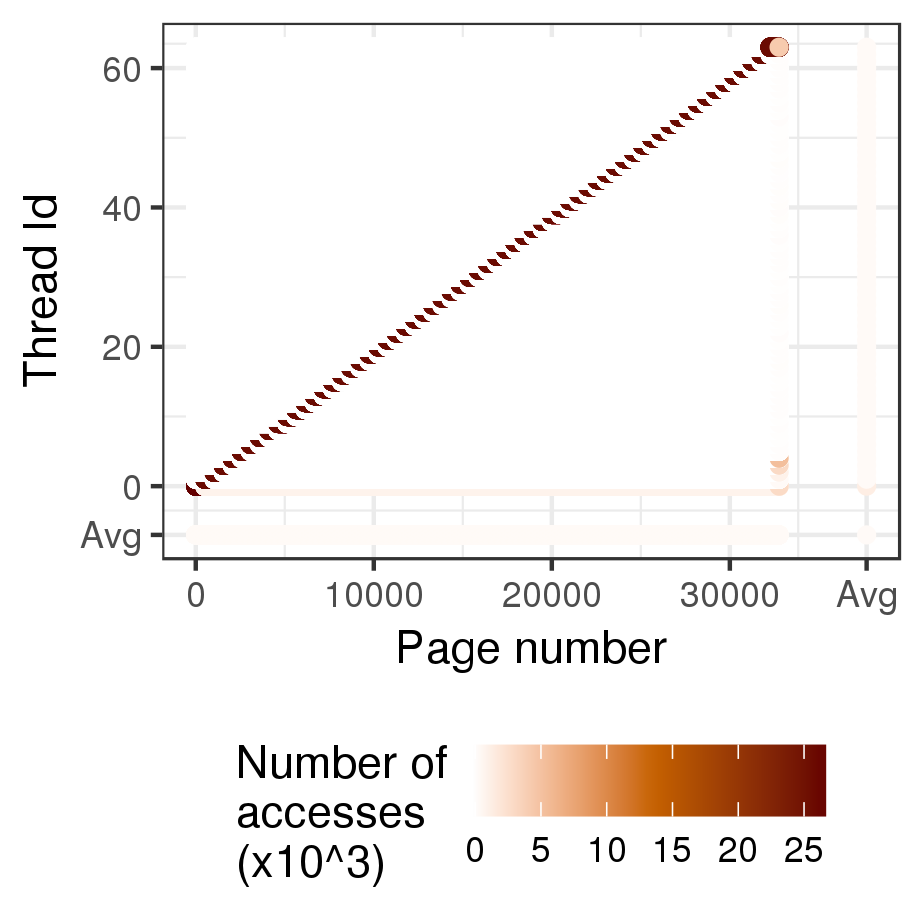
\includegraphics[width=\linewidth]{tabarnac/is_b_ka_dist_m.png}
            \end{column}
            \begin{column}{.45\linewidth}
                \centering
                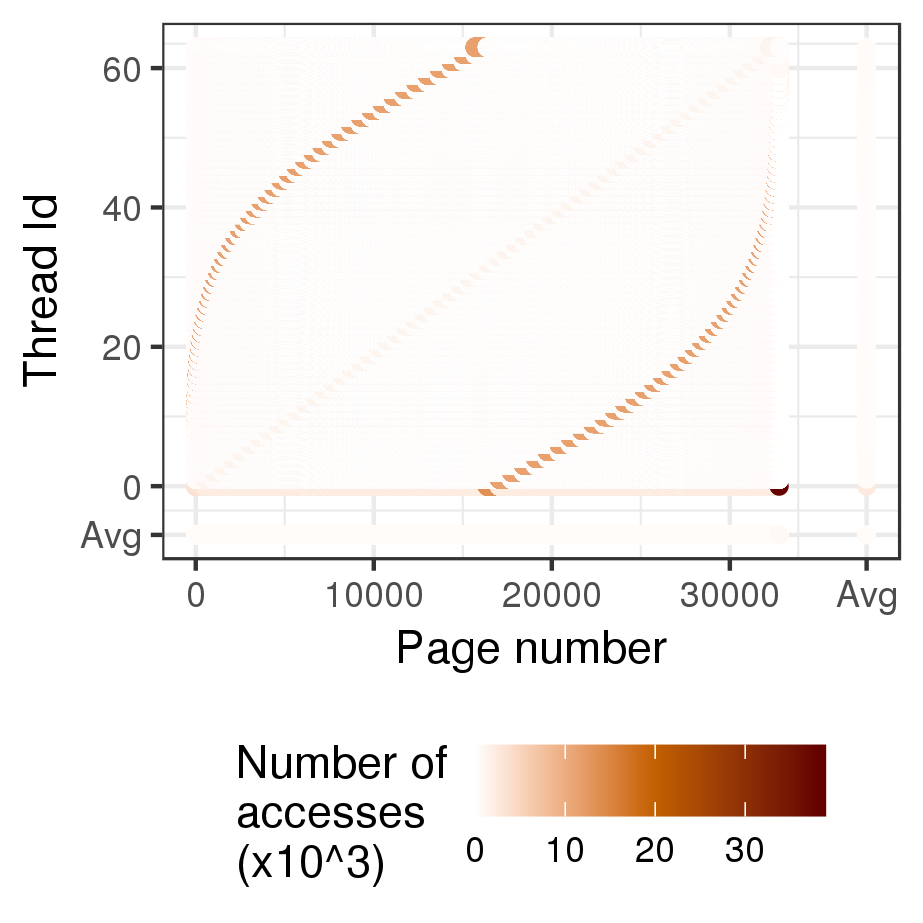
\includegraphics[width=\linewidth]{tabarnac/is_b_kb2_dist_m.png}
            \end{column}
        \end{columns}
    }{
        \centering
        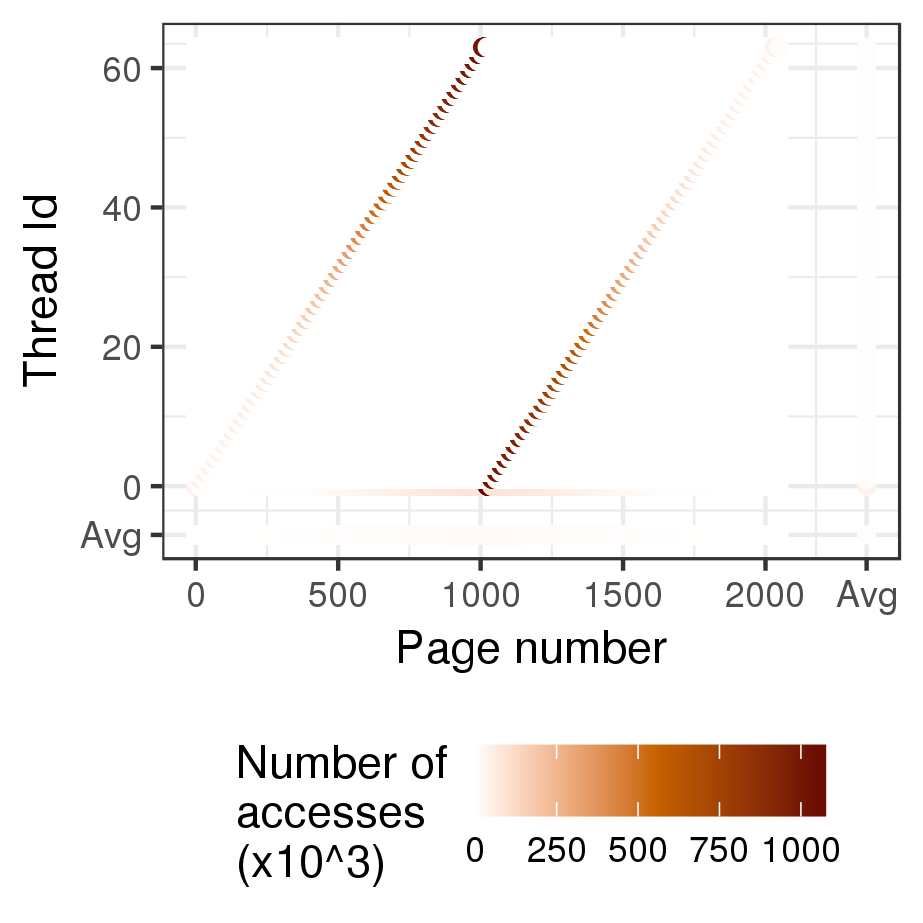
\includegraphics[width=.65\linewidth]{tabarnac/is_b_kb1_dist_m.png}
    }
    \pause
\end{frame}

\begin{frame}{Evaluation setup}
    \begin{block}{Machine}
        64 thread / 4 nodes NUMA machine
    \end{block}
    \pause
    \begin{block}{Optimization method}
        \begin{itemize}
            \item Base: Simple operating system
            \item Numa Balancing: Adaptive page mapping tool
            \item Interleave: Static mapping policy
        \end{itemize}
    \end{block}
    \pause
    \begin{alertblock}{Scheduling}
        \begin{itemize}
            \item Dynamic: default
            \item Cyclic: static
            \item Fair: ours
        \end{itemize}
    \end{alertblock}
\end{frame}

\begin{frame}{Results}
    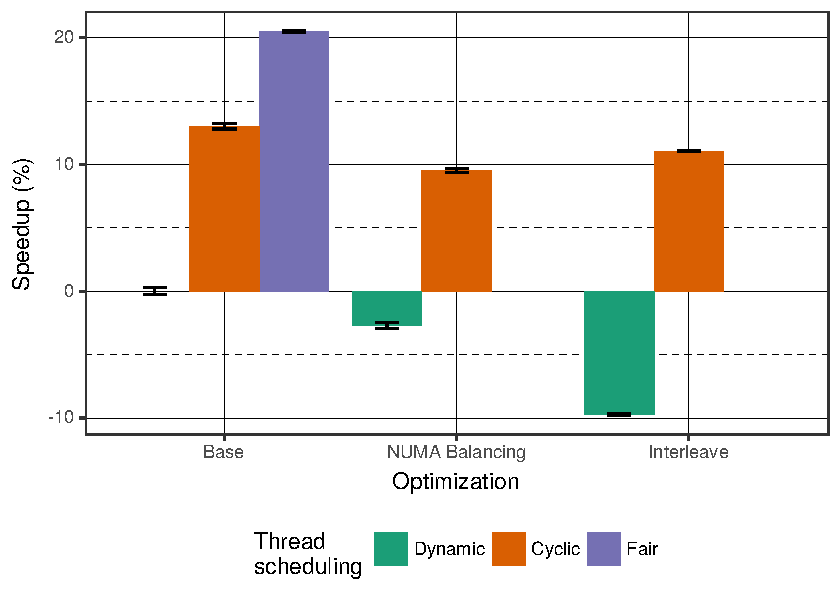
\includegraphics[width=\linewidth]{tabarnac/slides/is_exectime}
\end{frame}


\begin{frame}{Conclusions on Tabarnac}
    \begin{itemize}
        \item Collaboration with M. Diener, UFRGS, P.O.A, Brasil
        \item Improved trace collection tool
        \item Meaningful R visualization
        \item Significant performance gain on NPB IS
        \item<alert@1> Published at VPA'15~\cite{Beniamine15TABARNAC}
    \end{itemize}
    \uncover<2->{
        \begin{alertblock}{Limitations}
            \begin{itemize}
                \item No temporal informations
                \item Cannot detect precise sharing
            \end{itemize}
        \end{alertblock}
    }
\end{frame}

\section{Moca: Collecting and analyzing fine grained traces}

\subsection{Design}

\begin{frame}{Main principles}
    \begin{block}{Goals}
        \begin{itemize}
            \item Fine grained memory traces
            \item Reasonable overhead
            \item Limit impact on thread scheduling
        \end{itemize}
    \end{block}
    \pause
    \begin{alertblock}{Mechanism}
        Page faults interception and injection
    \end{alertblock}
\end{frame}

\begin{frame}{Main components}
    \begin{alertblock}{Linux kernel module}
        \begin{itemize}
            \item Monitor all threads of an application
            \item Intercept page faults
            \item Periodically injects false page faults
            \item Keep the recent trace (kernel space)
        \end{itemize}
    \end{alertblock}
    \uncover<2->{
        \begin{block}{User space process}
            \begin{itemize}
                \item Run application with context library
                \item Run application with kernel module loaded
                \item Periodically flush trace to disk
            \end{itemize}
        \end{block}
    }
\end{frame}

\begin{frame}{Managing data in kernel space}
    \centering
    \resizebox{!}{.85\textheight}{
        \pgfdeclarelayer{background}
\pgfdeclarelayer{bg1}
\pgfdeclarelayer{foreground}
\pgfsetlayers{background,bg1,main,foreground}

\definecolor{logcolor}{HTML}{FDAE61}
\definecolor{moncolor}{HTML}{FF1922}%FF000A: too dark for print
\definecolor{pfcolor} {HTML}{3B8ECC}
\definecolor{callcolor}{HTML}{FFFFBF}
\definecolor{dtcolorL}{HTML}{ABD9E9}
\colorlet{dtcolor}{dtcolorL!25}

\tikzstyle{handler} = [rectangle, draw, fill=callcolor,
text width=4em, text badly centered]
\tikzstyle{handlerI} = [diamond, text badly centered]
\tikzstyle{data} = [rectangle, draw, fill=dtcolor,
text width=4em, text centered, rounded corners]
\tikzstyle{Chunk} = [rectangle, draw,rounded corners]
\tikzstyle{dataL} = [rectangle, draw, fill=dtcolorL,
text width=4em, text centered, rounded corners]
\tikzstyle{entity} = [draw, ellipse, text centered,
text width=5em]
\tikzstyle{line} = [very thick,align=center]
\tikzstyle{pf} = [fill=pfcolor,solid]
\tikzstyle{log} = [fill=logcolor,dotted]
\tikzstyle{mon} = [fill=moncolor,dashed]
\tikzstyle{monA} = [-latex,line,dashed,moncolor]
\tikzstyle{pfA} =  [-latex,line,solid,pfcolor]
\tikzstyle{pfAI} =  [line,solid,pfcolor]
\tikzstyle{logA} = [-latex,dotted,line,logcolor]

\tikzset{
    basic box/.style = {
        shape = rectangle,
        draw,
    rounded corners},
    filled box/.style = {
        shape = rectangle,
        draw  = #1,
        fill  = #1,
    rounded corners},
    header node/.style = {
    %Minimum Width = header nodes,
        font          = \strut\large\ttfamily,
        text depth    = +0pt,
        fill          = #1,
    draw},
    header/.style n args={2}{%
        inner ysep = +1.5em,
        append after command = {
            \pgfextra{\let\TikZlastnode\tikzlastnode}
            node [header node=#2] (header-\TikZlastnode) at (\TikZlastnode.north) {#1}
      %node %[span = (\TikZlastnode)(header-\TikZlastnode)]
       % at (fit bounding box) (h-\TikZlastnode) {}
        }
    },
    footer node/.style = {
    %Minimum Width = header nodes,
        font          = \strut\large\ttfamily,
        text depth    = +0pt,
        fill          = #1,
    draw},
    footer/.style n args={2}{%
        inner ysep = +1.5em,
        append after command = {
            \pgfextra{\let\TikZlastnode\tikzlastnode}
            node [header node=#2] (header-\TikZlastnode) at (\TikZlastnode.south) {#1}
      %node %[span = (\TikZlastnode)(header-\TikZlastnode)]
       % at (fit bounding box) (h-\TikZlastnode) {}
        }
    },
    hv/.style = {to path = {-|(\tikztotarget)\tikztonodes}},
    vh/.style = {to path = {|-(\tikztotarget)\tikztonodes}},
    fat blue line/.style = {ultra thick, blue}
}



\begin{tikzpicture}[font=\small,scale=.73, each node/.style={minimum width=1em}]
    % Node placement
    \begin{pgfonlayer}{foreground}
        \node [Chunk] (ch3) at (0,0)        {Chunk3 empty};
        \node [Chunk] (ch2) at (0,-1)       {Chunk2 current};
        \node [Chunk] (ch1) at (0,-2)       {Chunk1 ending};
        \node [Chunk] (ch0) at (0,-3)       {Chunk0 completed};
        \node [Chunk] (cur) at (3,-1.5)   {current};

        \draw [line,->] (cur.north) |- (ch2.east);
    \end{pgfonlayer}

    \node [fit=(cur) (ch0) (ch1) (ch2) (ch3),filled box=dtcolor,
    header={Trace (1 Task)}{dtcolor!50}] (Tr) {};

    \node [data] (PfL) at (8,-1) {False Page fault map};
    \node [data] (TL)  at (12,-1) {Tasks map};


    \uncover<9->{
        \node[handler] (Flh) at (1,-5.5) {Read callback};
    }
    \uncover<2->{
        \node[handler] (PfH) at (10,-4.5) {page fault handler};
    }


    \uncover<8->{
        \node[entity,log] (F) at (1,-8) {Logging Process (userspace)};
    }
    \uncover<5->{
        \node[entity,mon] (M) at (6,-8) {Monitor thread (kernel)};
    }


    \begin{pgfonlayer}{background}
        \node[fit=(F) (M) (cur) (Flh) (PfH) (Tr) (PfL)(TL),header={Moca}{white},basic box] (Moca) {};
    \end{pgfonlayer}

    \node[entity,text width=5.5em,pf] (T) at (12,-14) {Tasks\\(user/kernel\\thread/process)};

    \node [dataL] (pgt)  at (6,-14)     {Page table (kernel)};
    \node [dataL] (proc) at (2,-14)     {/proc file (kernel)};
    \node [dataL] (file) at (-2,-14)     {File (userspace)};

    \begin{pgfonlayer}{background}
        \node[fit=(file) (proc) (pgt) (T),footer={Linux}{white} ,basic box=red,
        %below=1.5em of Moca
        ] (Linux) {};
    \end{pgfonlayer}

    % Edges

    %% Loging process
    \uncover<8->{
        \path[logA] (F.south) edge[in=140,out=270] node[right] {read} (proc.west);
    }
    \uncover<9->{
        \path[logA] (proc.north) edge[in=-20,out=70]  node[pos=.2,left] {triggers} (Flh.east);
    }
    \uncover<10->{
        \path[logA] (Flh.north) edge[out=90,in=270] node[pos=.2,left] {read write} (ch0.south);

        \path[logA] (Flh.west) edge[in=100,out=230] node[pos=.1,left] {write} (file.north);
    }

    % Page faults
    \uncover<2->{
        \path[pfA] (T)   edge[out=70,in=-70] node[pos=.2,right] {triggers} ($(PfH.south)+(1,0)$);
        \coordinate (inv2) at ($(M.south)-(0,0.5)$);
        \path[pfA] (PfH.north) edge node[right] {read \\ (write)} (TL.south);
    }

    \uncover<3->{
        \coordinate (inv) at (8.5,0.5);
        \path[pfAI] (PfH.north) edge[out=100,in=-10] (inv);
        \path[pfA]  (inv)     edge[out=170,in=20] node[pos=.1,above] {write} ($(ch2.east)+(0,0.2)$);
    }

    \uncover<4->{
        \path[pfA] (PfH.south) edge[out=-90, in=90] node[pos=.8,right] {read / write}(pgt.north);
        \path[pfA] (PfH.north) edge[out=160,in=310] node[pos=.8,right] {read} ($(PfL.south)+(0.2,0)$);

    }

    %Monitor
    \uncover<5->{
        \path[monA] (M.north) edge[out=110,in=-30] node[pos=.6,left] {write} (cur.east);
    }
    \uncover<6->{
        \path[monA] (M.north) edge[out=170,in=-10] node[pos=.5,left] {read} (ch1.east);
    }
    \uncover<7->{
        \path[monA] (M.north) edge[out=70,in=290] node[pos=.2,right] {write} (PfL.south);
        \path[monA] (M)  edge[out=-130,in=110] node[pos=.8,left] {write} ($(pgt.north)-(.6,0)$);

    }
\end{tikzpicture}


    }
\end{frame}

\begin{frame}{Handling page faults}
    \centering
    \resizebox{!}{.7\textheight}{
        %!TEX encoding=UTF-8 Unicode

\tikzstyle{decision} = [rectangle, draw, fill=orange!30,text centered,
text width=6.5em]
\tikzstyle{mblock} = [rectangle, draw, fill=blue!25,text centered, rounded corners, node distance=3cm, minimum height=3em]
\tikzstyle{lblock} = [rectangle, draw, fill=blue!10, text centered, rounded corners, node distance=3cm, minimum height=3em]
\tikzstyle{line} = [draw, -latex,thick]

\tikzset{
  basic box/.style = {
    shape = rectangle,
    draw,
    rounded corners},
  header node/.style = {
    %Minimum Width = header nodes,
    font          = \strut\large\ttfamily,
    text depth    = +0pt,
    fill          = #1,
    draw},
    header/.style n args={2}{%
    inner ysep = +2em,
    append after command = {
      \pgfextra{\let\TikZlastnode\tikzlastnode}
      node [header node=#2] (header-\TikZlastnode) at (\TikZlastnode.north) {#1}
      %node %[span = (\TikZlastnode)(header-\TikZlastnode)]
       % at (fit bounding box) (h-\TikZlastnode) {}
    }
  },
}

\newcommand*{\StrikeThruDistance}{0.15cm}%
%\newcommand*{\StrikeThru}{\StrikeThruDistance,\StrikeThruDistance}%
\tikzset{strike thru arrow/.style={
        decoration={markings, mark=at position 0.5 with {
            \draw [black, very thick,solid,-]
                    ++ (-\StrikeThruDistance,-\StrikeThruDistance)
                    -- ( \StrikeThruDistance, \StrikeThruDistance);
            \draw [black, very thick,solid,-]
                    ++ ( \StrikeThruDistance,-\StrikeThruDistance)
                    -- ( -\StrikeThruDistance, \StrikeThruDistance);
                } },
                    postaction={decorate},
                                    }
        }

    \begin{tikzpicture}[scale=0.8]

        \node [lblock]   (pf)  at (0,0) {PageFault(task, @)};

        \node [lblock]   (hpf)  at (0,-5) {HandleFault(task,@)};

        \node [lblock]   (resume)   at (0,-9){Resume execution};

        \uncover<2->{
            \node [mblock]   (pfi) at (10,0) {InterceptPageFault(task,@)};

            \node [decision] (mon) at (10,-2) {Is task monitored ?};

        }
        \uncover<3->{
            \node [decision] (shou) at (5,-3) {Should we monitor it ?};
            \node [mblock] (Add)  at (10,-5) {AddToChunk(task,@)};
        }

        \uncover<4->{
            \node [mblock] (Add1) at (5,-5) {Monitor(task)};
        }

        \uncover<5->{
            \node [decision] (sfix)     at (10,-7) {Is it a false page fault ?};
        }

        \uncover<6->{
            \node [mblock]   (fix)      at (10,-9) {FixFalsePageFault(task,@)};

        }
        \node[fit=(pfi) (shou) (fix),header={Moca}{white},basic box] (Moca) {};
        \node[fit=(pf) (hpf) (resume),header={Linux}{white},basic box] (OS) {};

        \only<1>{
            \draw [line] (pf) -- (hpf);
        }
        \path [line] (hpf) -- (resume);

        \only<2->{
            \path [line] (pf.south) -- ($(pf.south)+(0,-.4)$) --
            ($(pf.south)+(5,-.4)$)  -- ($(pfi.north)+(-5,.4)$) --
            ($(pfi.north)+(0,.4)$) -- (pfi.north);

            \draw [-latex, strike thru arrow,dashed] (pf) -- (hpf);

            \path [line] (pfi.south) -- (mon.north);
        }


        \only<3->{

            \path [line] (mon.west) -- node [pos=.2,above] {No} ($(mon)+(-5,0)$)
            -- (shou.north);
            \path [line] (mon.south) -- node [pos=.2,right] {Yes} (Add.north);
        }
        \only<4->{

            \path [line] (shou.west)  -- node [pos=.9,above] {No} ($(shou)+(-2.25,0)$)
            -- ($(shou)+(-2.25,-.5)$) -- ($(hpf)+(0,1.5)$) -- (hpf.north);

            \path [line] (shou.south) -- node [right] {Yes} (Add1.north);

            \path [line] (Add1.south) -- ($(Add1.south)+(0,-.5)$)
            -- ($(Add1.south)+(2,-.5)$) -- ($(Add.north)+(-3,1)$)
            -- ($(Add.north)+(0,1)$) -- (Add.north);

        }
        \only<5->{
            \path [line] (Add.south) -- (sfix);

        }\only<6->{
            \path [line] (sfix.west) -- node [pos=.1,above] {No}
            ($(sfix)+(-7.25,0)$) -- ($(sfix)+(-7.25,3.5)$)
            -- ($(hpf)+(0,1.5)$) -- (hpf.north);

            \path [line] (sfix.south) -- node [right] {Yes} (fix.north);
        }
        \only<7->{
            \path [line] (fix.south) -- ($(fix.south)+(0,-.5)$)
            -- ($(fix.south)+(-7.25,-.5)$) -- ($(fix)+(-7.25,1.5)$)
            -- ($(resume)+(0,1.5)$) --(resume.north);
        }

    \end{tikzpicture}


% vim: et si sta lbr  sw=4 ts=4 spelllang=en_us


    }
\end{frame}

\subsection{Experimental evaluation}

\begin{frame}{Tools comparison}
    \small
    \begin{tabular}{lcccc}
        \toprule
         & \textbf{Moca} & \textbf{Tabarnac} & \textbf{Mitos} & \textbf{MemProf} \\
            \midrule
            \textbf{Design} & & & &\\
            \midrule
            Mechanisms   & Page faults  & Instrumentation & PEBS & IBS \\
            Architecture & \textbf{Any} & Intel (AMD) & Intel & AMD   \\
            \midrule
            \textbf{Completeness} & & & &\\
            \midrule
            Granularity & \textbf{Address} & Page          & \textbf{Address} & \textbf{Address} \\
            Superset          & \textbf{Page} & \textbf{Page} & None             & None             \\
            \midrule
            \textbf{Detail} & & & &\\
            \midrule
            Temporal data & \textbf{Yes} & No          & \textbf{Yes} & \textbf{Yes} \\
            CPU location  & \textbf{Yes} & No          & \textbf{Yes} & \textbf{Yes} \\
            Nature        & \textbf{Yes} &\textbf{Yes} & Yes         & Yes       \\
        \bottomrule
    \end{tabular}
\end{frame}

\begin{frame}{Benchmarks}
    \small
    \begin{tabular}{lrll}
        \toprule
        \textbf{Name} & \textbf{Footprint} & \textbf{Description} & \textbf{Group} \\
        \midrule
        \IS & \SI{132}{Mib} & Integer Sort  &
        \multirow{4}{*}{Memory Intensive}\\
        \CG & \si{125}{Mib} & Conjugate Gradient & \\
        \MG & \si{508}{Mib}& Multi-grid & \\
        \FT & \si{398}{Mib}& Discrete 3D FFT & \\
        \midrule
        \UA & \si{112}{Mib}& Unstructured Adaptive mesh &
        \multirow{2}{*}{Unstructured} \\
        \DC & $1.46$Gib & Data Cube & \\
        \midrule
        \BT & \si{120}{Mib}& Block Tri-diagonal solver &
        \multirow{3}{*}{Pseudo Apps} \\
        \SP & \si{122}{Mib}& Scalar Penta-diagonal solver & \\
        \LU & \si{118}{Mib}& Lower-Upper Gauss-Seidel solver & \\
        \midrule
        \EP & \si{78}{Mib}& Embarrassingly parallel & CPU bound\\
        \bottomrule
    \end{tabular}
\end{frame}

\begin{frame}{Percentage of captured pages}
        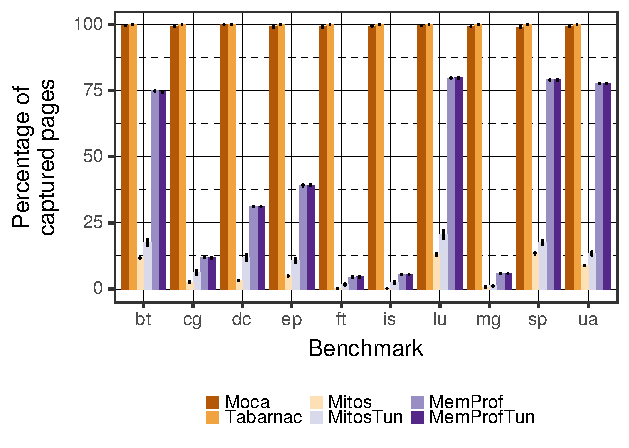
\includegraphics[width=\linewidth]{moca/slides/moca_pages_intel.pdf}
\end{frame}

\begin{frame}{Number of captured events}
        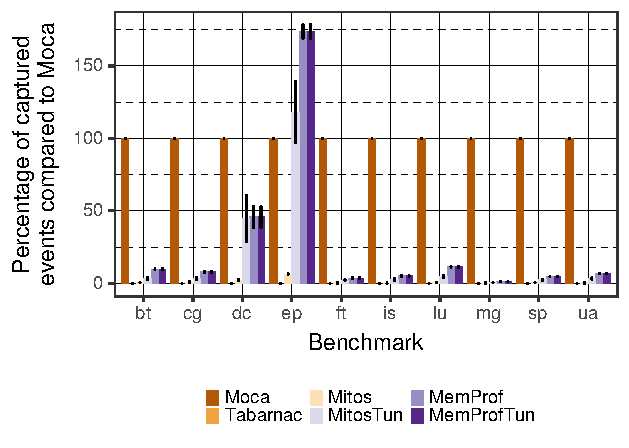
\includegraphics[width=\linewidth]{moca/slides/moca_addr_intel.pdf}
\end{frame}

\begin{frame}{Tracing overhead (intel)}
        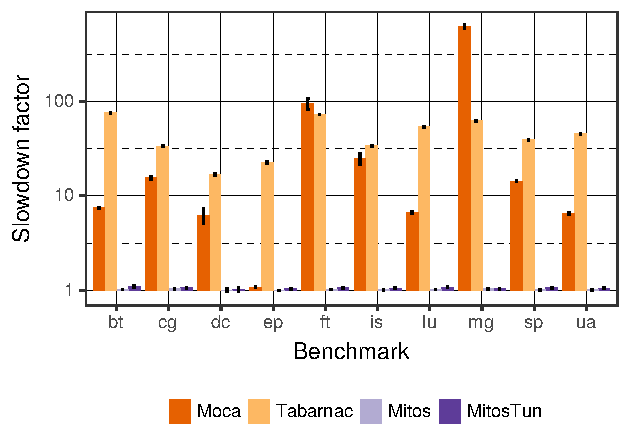
\includegraphics[width=\linewidth]{moca/slides/moca_overhead_intel.pdf}
\end{frame}

\section{Conclusions and perspectives}

\begin{frame}{Conclusions}
    \begin{alertblock}{}
        How can we analyze the memory behavior of an application to optimize its performances ?
    \end{alertblock}
    \pause
    \begin{block}{Tabarnac~\cite{Beniamine15TABARNAC}}
        \begin{enumerate}
            \item \textbf{Tace collection:} No temporal informations
            \item \textbf{Visualization:} Simple yet meaningful
            \item \textbf{Optimization:} To 20\% performance gain on NPB IS
        \end{enumerate}           
    \end{block}
    \pause
    \begin{alertblock}{Moca~\cite{Beniamine15Memory,Beniamine16Moca}}
        \begin{enumerate}
            \item \textbf{Trace collection:} Complete, detailed, precise
            \item \textbf{Visualization:} Encouraging preliminary results
            \item \textbf{Optimization:} Still a work in progress
        \end{enumerate}          
    \end{alertblock}
\end{frame}

\begin{frame}{Perspectives}
    \begin{block}{Short term}
        \begin{itemize}
            \item Use Moca traces to understand Intel MKL performaances
            \item Analyze other real applications
            \item Couple Moca traces with performances counters
        \end{itemize}
    \end{block}
    \pause
    \begin{alertblock}{Long term}
        \begin{itemize}
            \item Higher level trace visualization for Moca
            \item Similar tools for GPU / Accelerators
        \end{itemize}
    \end{alertblock}
\end{frame}

\newcounter{finalframe}
\setcounter{finalframe}{\value{framenumber}}
%Last numbered frame go here

\begin{frame}{}
    \centering
    \Huge
    Thank you
\end{frame}
%=============================================================================

%=============================================================================
%Uncomment next lines for uncounted backup slides & biblio
%========================= Backup slides =====================================
\section*{Hidden slides}
%put this line before each frame
%\setcounter{framenumber}{\value{finalframe}}

\subsection*{Related work}
\setcounter{framenumber}{\value{finalframe}}
\begin{frame}{Generic performance analysis tools}
    \begin{block}{Low level trace collection libraries}
        \begin{itemize}
            \item PAPI~\cite{Browne00Portable}
            \item Likwid~\cite{Treibig10LIKWID}
        \end{itemize}
    \end{block}
    \pause
    \begin{block}{Higher level tools}
        \begin{itemize}
            \item PARAVER~\cite{Pillet95PARAVER}
            \item MAQAO~\cite{Djoudi05MAQAO}
            \item VTune~\cite{Reinders05VTune}
            \item HPCToolkit~\cite{Adhianto10HPCTOOLKIT}
            \item \ldots
        \end{itemize}
    \end{block}
    \pause
    \begin{alertblock}{Limitations}
        Focus on CPU point of view
    \end{alertblock}
\end{frame}

\subsection*{Tabarnac}

\setcounter{framenumber}{\value{finalframe}}
\begin{frame}{Experimental setup}
    \small
    \centering
    \begin{tabular}{lccccc}
        \toprule
        & \multicolumn{5}{c}{\textbf{Hardware totals}}\\
        \cmidrule(lr){2-6}
        & Nodes & Threads & Vendor & Model & Memory \\
        \cmidrule(lr){2-6}
        \texttt{Turing}   & $4$ & $64$ & Intel & Xeon X7550   & \SI{128}{Gib} \\
        \texttt{Idfreeze} & $8$ & $48$ & AMD   & Opteron 6174 & \SI{256}{Gib}\\
        \midrule
        & \multicolumn{5}{c}{\textbf{Hardware per node}}\\
        \cmidrule(lr){2-6}
        & Cores & Threads & Frequency & L3 Cache & Memory \\
        \cmidrule(lr){2-6}
        \texttt{Turing}   & $8$ & $16$ & \SI{2.00}{Ghz}& \SI{18}{Mib} & \SI{32}{Gib} \\
        \texttt{Idfreeze} & $6$ & $6$  & \SI{2.20}{Ghz}& \SI{12}{Mib} & \SI{32}{Gib}\\
        \midrule
        & \multicolumn{5}{c}{\textbf{Software}}\\
        \cmidrule(lr){2-6}
        & Kernel & \multicolumn{2}{c}{Distribution} &
        \multicolumn{2}{c}{Bios configurations} \\
        \cmidrule(lr){2-6}
        \texttt{Turing}   & Linux 3.13 & \multicolumn{2}{c}{Ubuntu 12.04} &
        \multicolumn{2}{c}{Hyper threading} \\
        \texttt{Idfreeze} & Linux 3.2 & \multicolumn{2}{c}{Debian Jessie} &
        \multicolumn{2}{c}{No hyper threading}\\
        \bottomrule
    \end{tabular}
\end{frame}

\setcounter{framenumber}{\value{finalframe}}
\begin{frame}{Tabarnac overhead}
    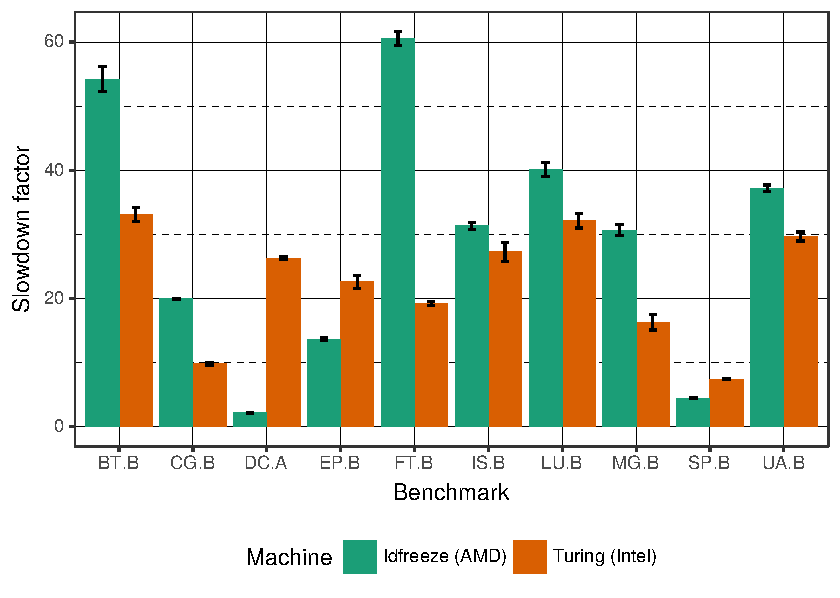
\includegraphics[width=\linewidth]{tabarnac/slides/tool-ovh.pdf}
\end{frame}

\subsection*{Moca}

\setcounter{framenumber}{\value{finalframe}}
\begin{frame}{Experimental setup}
    \small
    \begin{tabular}{lllllllllll}
        \toprule
        & \multicolumn{5}{c}{\textbf{Hardware totals}}\\
        \cmidrule(lr){2-6}
        & Nodes & Threads & \multicolumn{2}{c}{CPU} & Memory \\
        \cmidrule(lr){2-6}
        \texttt{Edel}    & $2$ & $8$  & \multicolumn{2}{c}{Intel Xeon E5520}      & \SI{24}{Gib} \\
        \texttt{StRemi} & $2$ & $24$ & \multicolumn{2}{c}{AMD Opteron 6164 HE }& \SI{48}{Gib} \\
        \midrule
        & \multicolumn{5}{c}{\textbf{Hardware per node}}\\
        \cmidrule(lr){2-6}
        & Cores & Threads & Frequency & L3 Cache & Memory \\
        \cmidrule(lr){2-6}
        \texttt{Edel}   & $4$  & $4$   & \SI{2.27}{Ghz}& \SI{8}{Mib}  & \SI{12}{Gib} \\
        \texttt{StRemi} & $12$ & $12$  & \SI{1.70}{Ghz}& \SI{12}{Mib} & \SI{24}{Gib}\\
        \midrule
        & \multicolumn{5}{c}{\textbf{Software}}\\
        \cmidrule(lr){2-6}
        & \multicolumn{2}{c}{Distribution} & Kernel &
            \multicolumn{2}{c}{Bios configurations} \\
        \cmidrule(lr){2-6}
        \texttt{Turing}   & \multicolumn{2}{c}{Debian Jessie} & Linux 3.16.0-4 &
            \multicolumn{2}{c}{No hyper threading} \\
        \texttt{Idfreeze} & \multicolumn{2}{c}{Debian Jessie} & Linux 3.16.0-4 &
            \multicolumn{2}{c}{No hyper threading}\\
        \bottomrule
    \end{tabular}
\end{frame}

\setcounter{framenumber}{\value{finalframe}}
\begin{frame}{Parameters evaluation}
   \alt<1>{
    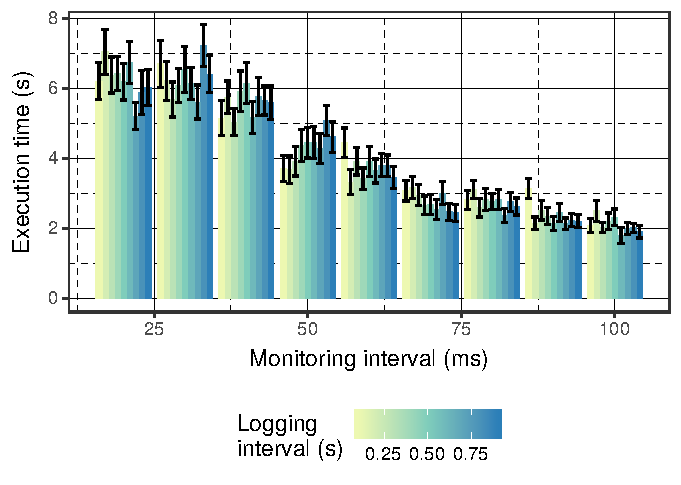
\includegraphics[width=\linewidth]{moca/slides/moca_param.pdf}
    }{
        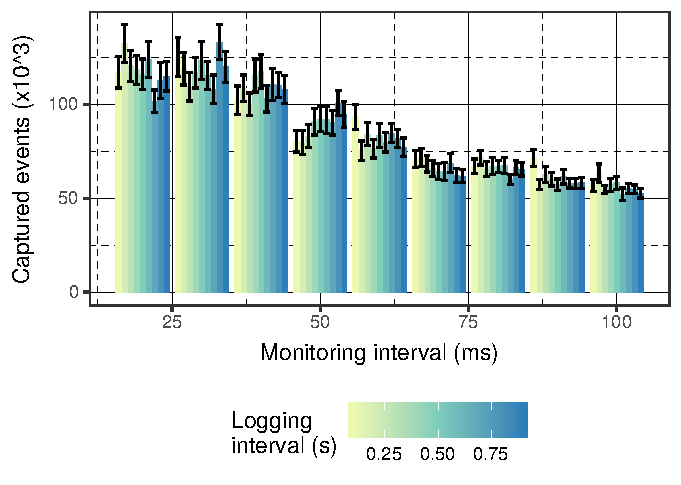
\includegraphics[width=\linewidth]{moca/slides/moca_param_events.pdf}
    }
    \pause
\end{frame}


\setcounter{framenumber}{\value{finalframe}}
\begin{frame}{Experimental results: tracing overhead (amd)}
        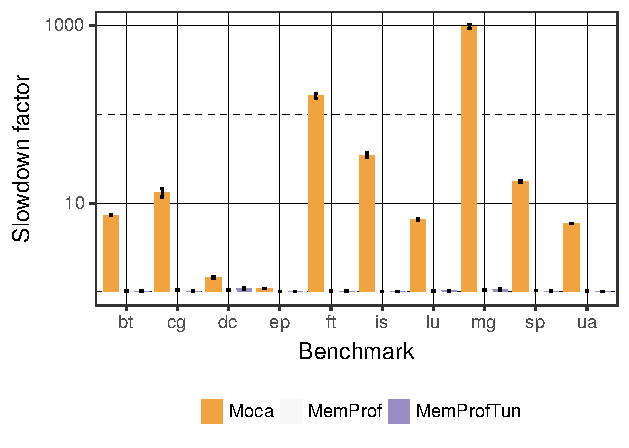
\includegraphics[width=\linewidth]{moca/slides/moca_overhead_amd.pdf}
\end{frame}

\subsection*{Visualizing and analyzing Moca traces}

\begin{frame}{FrameSoc and Ocelotl}
    \begin{block}{FrameSoc~\cite{Pagano14frameSoC}}
        \begin{itemize}
            \item Generic trace management tool
            \item Several visualization of a trace
            \item Designed for trace exploration
        \end{itemize}
    \end{block}
    \pause
    \begin{alertblock}{Ocelotl~\cite{Dosimont14Ocelotl}}
        \begin{itemize}
            \item FrameSoc Tool
            \item Aggregates trace aiming at reducing information loss
            \item Simple zoom and filters operations
        \end{itemize}
    \end{alertblock}
\end{frame}

\setcounter{framenumber}{\value{finalframe}}
\begin{frame}{Example: Matrix multiplication}
    \centering
    \alt<1>{
        \resizebox{.8\linewidth}{!}{
            % -
 %              DO WHAT THE FUCK YOU WANT TO PUBLIC LICENSE
 %                      Version 2, December 2004
 %   
 %   Copyright (C) 2016 Beniamine, David <David@Beniamine.net>
 %   Author: Beniamine, David <David@Beniamine.net>
 %   
 %   Everyone is permitted to copy and distribute verbatim or modified
 %   copies of this license document, and changing it is allowed as long
 %   as the name is changed.
 %   
 %              DO WHAT THE FUCK YOU WANT TO PUBLIC LICENSE
 %     TERMS AND CONDITIONS FOR COPYING, DISTRIBUTION AND MODIFICATION
 %   
 %    0. You just DO WHAT THE FUCK YOU WANT TO.
 %%

%!TEX encoding=UTF-8 Unicode
%Palette YlOrRd, 3 col
\definecolor{ColV}{HTML}{FFEDA0}
\definecolor{ColH}{HTML}{F03B20}

%Palette 4-class paired
\definecolor{Col0}{HTML}{A6CEE3}
\definecolor{Col1}{HTML}{1F78B4}
\definecolor{Col2}{HTML}{B2DF8A}
\definecolor{Col3}{HTML}{33A02C}


\pgfdeclarelayer{background}
\pgfdeclarelayer{foreground}
\pgfsetlayers{background,foreground}


\tikzstyle{PrimaryA}   = [-latex,very thick]
\tikzstyle{SecondaryA} = [-latex,very thick,dashed]
\tikzstyle{SwapA} = [latex-latex, thick,dotted]

\newcommand{\coli}[1]{\textcolor{ColI}{#1}}
\newcommand{\colj}[1]{\textcolor{ColJ}{#1}}
\newcommand{\colk}[1]{\textcolor{ColK}{#1}}

\newcommand{\Ta}{\textcolor{Col0}{Thread~1}\xspace}
\newcommand{\Tb}{\textcolor{Col1}{Thread~2}\xspace}
\newcommand{\Tc}{\textcolor{Col2}{Thread~3}\xspace}
\newcommand{\Td}{\textcolor{Col3}{Thread~4}\xspace}

\tikzset{
    algorithm/.style={
        shape=rectangle,
        alias=this,
        append after command = {
            \pgfextra{
              % Top and bottom lines
                \draw [] ($(this.north west)+(0,.5)$) -- ($(this.north east)+(0,.5)$);
                \node [anchor=west] at ($(this.north west)+(0,0.25)$) {\textbf{Algorithm} #1};
                \draw [] (this.north west) -- (this.north east);
                \draw [] (this.south west) -- (this.south east);
            }
        }
    },
    matgrid/.style args={#1#2}{
        %#1: name #2: size
        alias=this,
        append after command ={
            \pgfextra{
                \draw[very thin,loosely dotted,step=.5] (this) grid ($(this)+(#2,#2)$);
                \draw (this) rectangle ($(this)+(#2,#2)$);
                % Four corners
                \coordinate (m#1-00) at ($(this)+(0,0)$);
                \coordinate (m#1-0N) at ($(this)+(0,#2)$);
                \coordinate (m#1-N0) at ($(this)+(#2,0)$);
                \coordinate (m#1-NN) at ($(this)+(#2,#2)$);

                \coordinate(m#1-east) at ($(m#1-00)!.5!(m#1-0N)$);
                \coordinate(m#1-west) at ($(m#1-N0)!.5!(m#1-NN)$);
                \coordinate(m#1-north)  at ($(m#1-00)!.5!(m#1-N0)$);
                \coordinate(m#1-south)  at ($(m#1-0N)!.5!(m#1-NN)$);

                \node (#1) at ($(m#1-00)+(-.5,0)$){\textbf{#1}};

            }
        }
    }
}



\begin{tikzpicture}[font=\small]

    \begin{pgfonlayer}{background}

        \node[matgrid={A}{4}] at (0,0){};
        \node[matgrid={B}{4}] at (5,5){};
        \node[matgrid={C}{4}] at (5,0){};

    \end{pgfonlayer}

    % Indexes

    \begin{pgfonlayer}{foreground}
        %% A
        \draw[very thick,ColV] (mA-west) -- (mA-east);
        \draw[very thick,ColV] (mC-west) -- (mC-east);
        \draw[very thick,ColH] (mB-north) -- (mB-south);
        \draw[very thick,ColH] (mC-north) -- (mC-south);

        \node at ($(mA-east)!0.5!(mA-west)+(0,1)$) {\Ta and \Tb};
        \node at ($(mA-east)!0.5!(mA-west)+(0,-1)$) {\Tc and \Td};
 
        \node[text centered,text width=5em] at ($(mB-north)!0.5!(mB-south)+(-1,0)$) {\Ta and \Tc};
        \node[text centered,text width=5em] at ($(mB-north)!0.5!(mB-south)+(1,0)$) {\Tb and \Td};

        \node[text centered] at ($(mC-east)!0.5!(mC-west)+(-1,1)$)  {\Ta};
        \node[text centered] at ($(mC-east)!0.5!(mC-west)+(1,1)$)   {\Tb};
        \node[text centered] at ($(mC-east)!0.5!(mC-west)+(-1,-1)$) {\Tc};
        \node[text centered] at ($(mC-east)!0.5!(mC-west)+(1,-1)$)  {\Td};
    \end{pgfonlayer}

\end{tikzpicture}
% vim: et si sta lbr  sw=4 ts=4 spelllang=en_us

        }
    }{
        \alt<2>{
            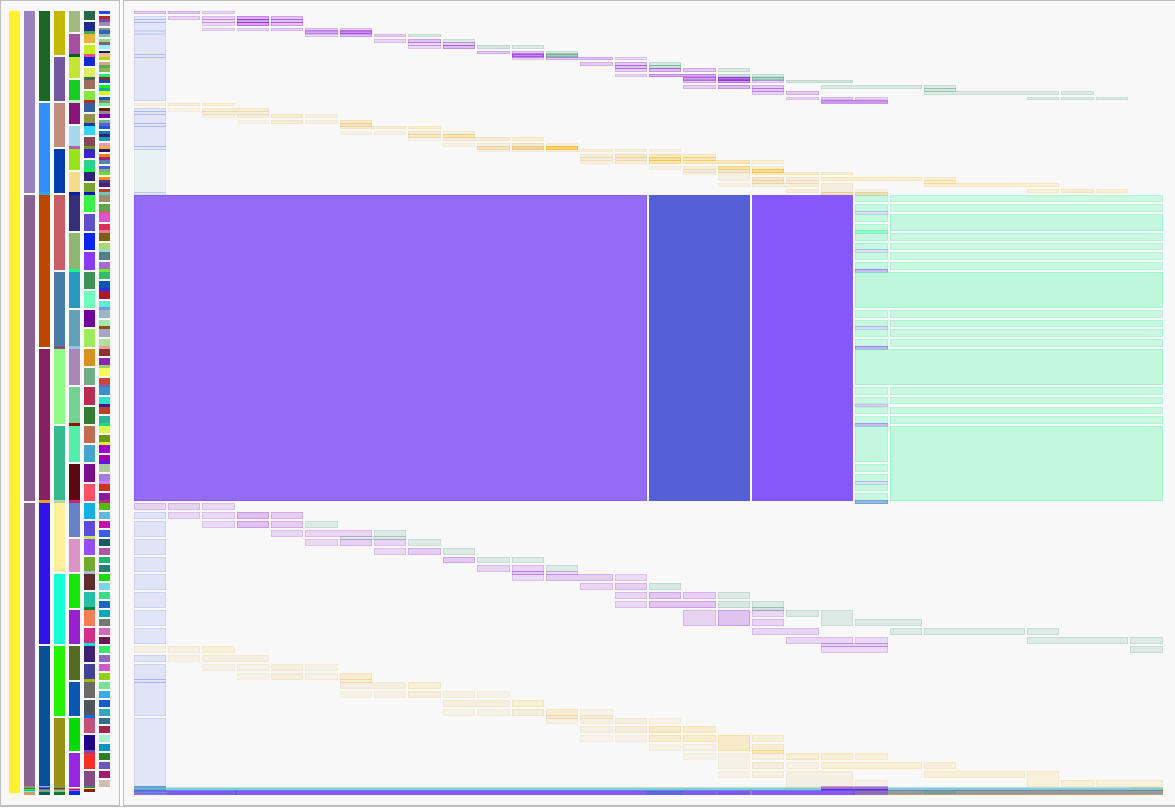
\includegraphics[width=\textwidth]{ocelotl/TaskView.png}
        }{
            \alt<3>{
                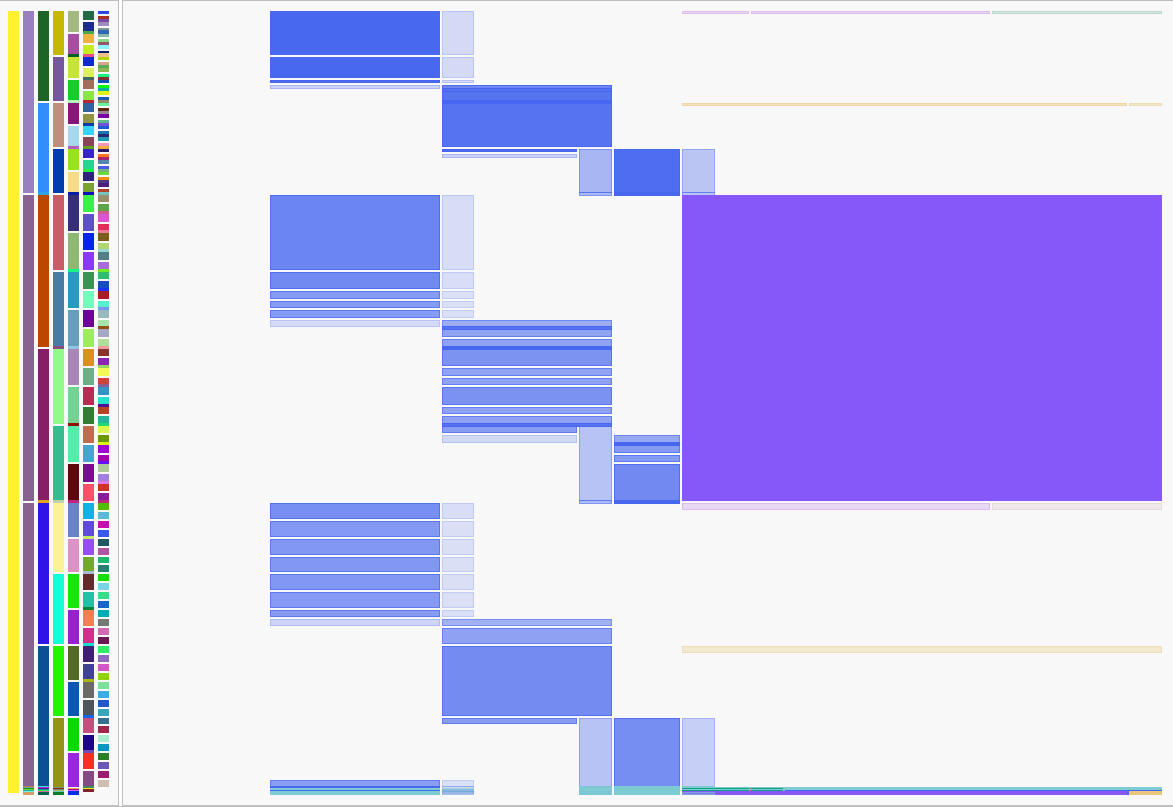
\includegraphics[width=\textwidth]{ocelotl/TaskView-zoom-init.png}
            }{
                \alt<4>{
                    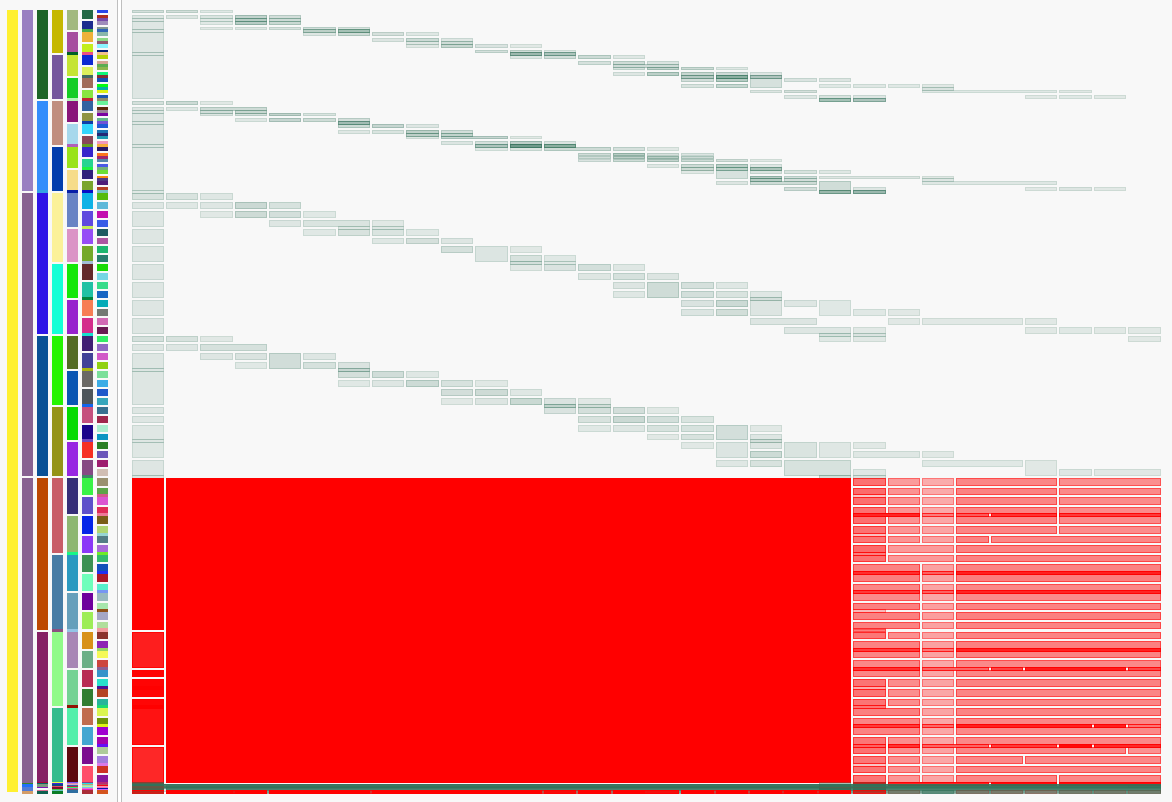
\includegraphics[width=\textwidth]{ocelotl/Sharing.png}
                }{
                    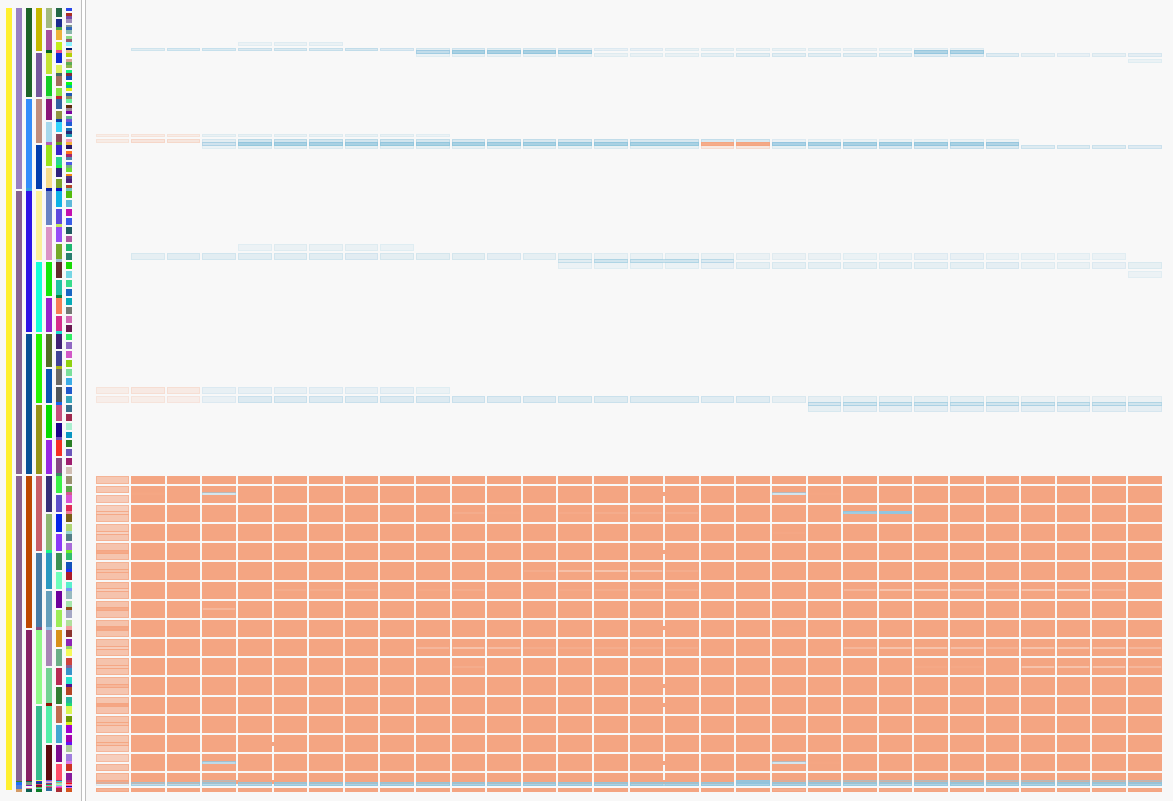
\includegraphics[width=\textwidth]{ocelotl/Sharing-zoom.png}
                }
            }
        }
    }
    \pause
    \pause
    \pause
    \pause
\end{frame}%

\begin{frame}{Limits}
    \begin{itemize}
        \item FrameSoc trace model not well suited for memory traces
        \item Interaction is too slow
        \item Hard to identify / filter by data structures
    \end{itemize}
\end{frame}

\begin{frame}{Programmatic approach}
    \begin{block}{Idea}
        \begin{itemize}
            \item Programmatic approach using R
            \item Org-mode labbook to record our analysis
            \item Reference visualizations inspired from Tabarnac ones
            \item Custom visualizations depending on the trace
        \end{itemize}
    \end{block}
\end{frame}

\setcounter{framenumber}{\value{finalframe}}
\begin{frame}{Example: dgetrf}
    \centering
    \alt<1>{
        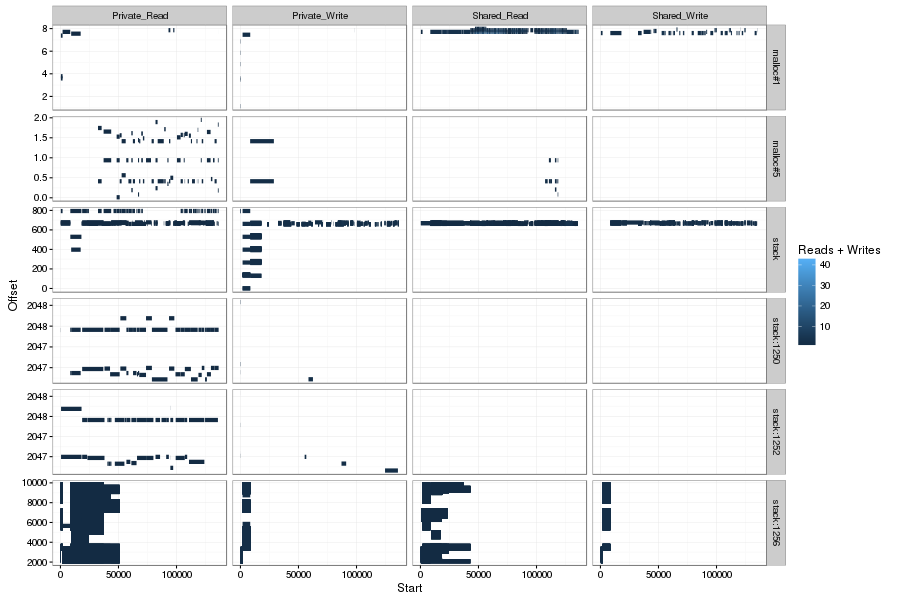
\includegraphics[width=\textwidth]{labbook-slides/intensity_Rw_dgetrf}
    }{
        \alt<2>{
            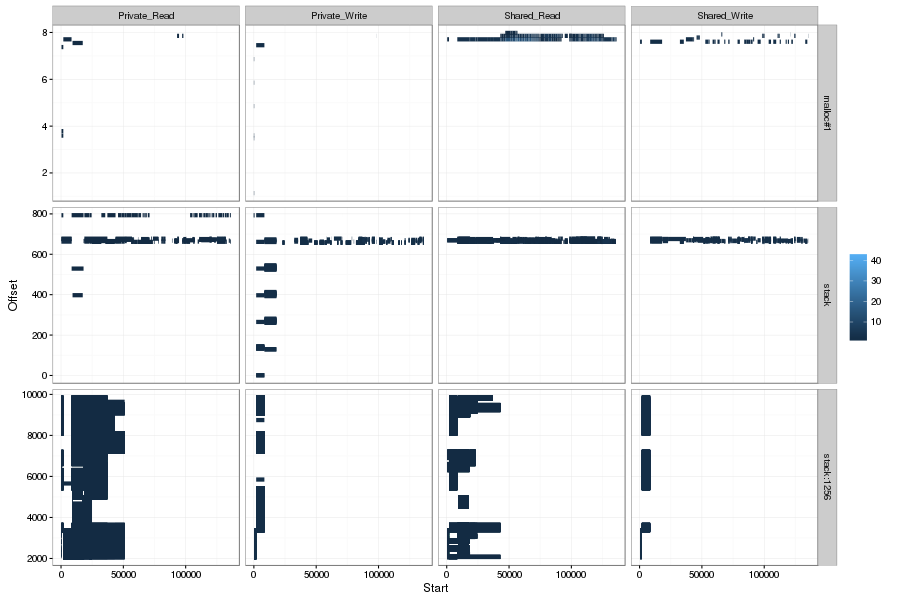
\includegraphics[width=\textwidth]{labbook-slides/intensity_RW_dgetrf_zoom}
        }{
            \alt<3>{
                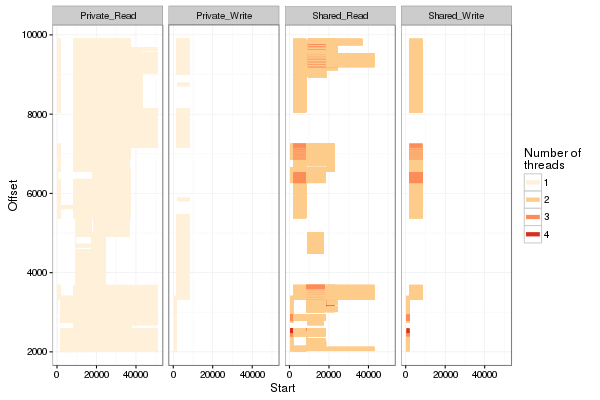
\includegraphics[width=\textwidth]{labbook-slides/intensity_Share_dgetrf_zoom-init}
            }{
                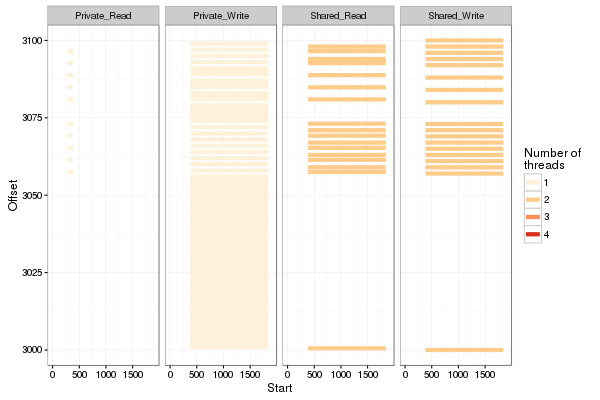
\includegraphics[width=\textwidth]{labbook-slides/intensity_Share_dgetrf_zoom-init1}
            }
        }
    }
    \pause
    \pause
    \pause
\end{frame}%

%=============================================================================

\section*{Bibliography}
%
\bibliographystyle{apalike}
\bibliography{biblio}


\end{document}
